% =====================================================================
%  Reasoning Models  --  a lecture on models that think before they
%  answer: chain of thought and why extra tokens buy computation,
%  search and verifiers, training with reinforcement learning on
%  verifiable rewards (STaR, GRPO, DeepSeek-R1, DAPO), distillation,
%  test-time compute and budgets, the 2026 landscape, the limits
%  (faithfulness, overthinking, jaggedness) and practice.
%  Same visual language as "The Transformer, Visually".
%
%  Compile:  pdflatex reasoning_models_tutorial.tex   (run twice)
%  Self-contained: every figure is TikZ/pgfplots source in this file.
%
%  Conventions
%   * \stage{n} before a frame sets the accent color and highlights the
%     matching chip in the footer strip.
%   * Numbers quoted from a paper or a vendor report name the source;
%     numbers labeled "derived" were computed from quoted ones; curves
%     labeled "illustrative" are sketches, not data; $^\dagger$ marks
%     vendor documentation, model cards, blogs and commentary.
% =====================================================================
\documentclass[aspectratio=169,11pt]{beamer}

% ---------- fonts ----------------------------------------------------
\usepackage[scaled=0.92]{helvet}        % Helvetica-like sans for text
\renewcommand{\ttdefault}{cmtt}         % Computer Modern mono for tokens
\usefonttheme[onlymath]{serif}          % classic serif math
\usepackage{amsmath,amssymb,bm}
\usepackage{booktabs,array}
\usepackage{graphicx}


% ---------- graphics -------------------------------------------------
\usepackage{tikz}
\usepackage{pgfplots}
\pgfplotsset{compat=1.17}
\usetikzlibrary{arrows.meta,positioning,calc,fit,backgrounds,
                decorations.pathreplacing,shapes.geometric}

% ---------- palette --------------------------------------------------
\definecolor{ink}{HTML}{1F2937}     % text, residual stream
\definecolor{muted}{HTML}{6B7280}   % secondary text
\definecolor{hair}{HTML}{D9DDE4}    % hairlines
\definecolor{paper}{HTML}{FCFCFA}   % slide background
\definecolor{tok}{HTML}{5F6F85}     % tokens / tokenizer
\definecolor{emb}{HTML}{0CA678}     % embeddings
\definecolor{posc}{HTML}{7048E8}     % positional information
\definecolor{attn}{HTML}{E8590C}    % attention
\definecolor{mlp}{HTML}{1C7ED6}     % MLP / feed-forward
\definecolor{norm}{HTML}{5C940D}    % normalization
\definecolor{outc}{HTML}{D6336C}     % unembedding / softmax / sampling
\definecolor{trn}{HTML}{9C6644}     % training and scaling
\colorlet{qc}{attn}                 % queries
\definecolor{kc}{HTML}{F59F00}      % keys
\definecolor{vc}{HTML}{1098AD}      % values
\colorlet{kct}{kc!70!black}         % key color, darkened for text
\colorlet{stagec}{ink}              % accent of the current stage

% ---------- beamer look ----------------------------------------------
\setbeamertemplate{navigation symbols}{}
\setbeamercolor{background canvas}{bg=paper}
\setbeamercolor{normal text}{fg=ink}
\setbeamercolor{frametitle}{fg=ink}
\setbeamersize{text margin left=8mm,text margin right=8mm}
\setbeamertemplate{itemize item}{\raisebox{0.25ex}{\tiny\color{stagec}$\blacksquare$}}
\setlength{\leftmargini}{1.1em}
\hyphenpenalty=10000 \exhyphenpenalty=10000   % no hyphenation on slides

% stage = which part of the pipeline the slide belongs to
\newcount\stageno \stageno=1
\newcommand{\stage}[1]{\global\stageno=#1\relax
  \ifcase#1\or\colorlet{stagec}{ink}\or\colorlet{stagec}{tok}%
  \or\colorlet{stagec}{emb}\or\colorlet{stagec}{attn}%
  \or\colorlet{stagec}{mlp}\or\colorlet{stagec}{posc}%
  \or\colorlet{stagec}{trn}\or\colorlet{stagec}{outc}%
  \or\colorlet{stagec}{vc}\or\colorlet{stagec}{ink}\fi}

\makeatletter
% title: accent bar + title + one-line claim (the frame subtitle)
\setbeamertemplate{frametitle}{%
  \nointerlineskip\vspace*{3.6mm}%
  \begin{tikzpicture}[x=1mm,y=1mm]
    \useasboundingbox (0,0) rectangle (144,10.5);
    \fill[stagec,rounded corners=0.5mm] (0,0.3) rectangle (1.5,10.2);
    \ifx\insertframesubtitle\@empty
      \node[anchor=west,inner sep=0,text=ink,
            font=\fontsize{15}{17}\selectfont\bfseries] at (4.2,5.2) {\insertframetitle};
    \else
      \node[anchor=west,inner sep=0,text=ink,
            font=\fontsize{15}{17}\selectfont\bfseries] at (4.2,7.1) {\insertframetitle};
      \node[anchor=west,inner sep=0,text=muted,
            font=\fontsize{8.6}{10}\selectfont] at (4.2,2.0) {\insertframesubtitle};
    \fi
  \end{tikzpicture}}
\makeatother

% footer: pipeline strip with the current stage lit, plus page number
\setbeamertemplate{footline}{%
  
\begin{tikzpicture}[x=1mm,y=1mm]
    \useasboundingbox (0,0) rectangle (160,7.2);
    \coordinate (c0) at (7.2,4.0);
    \foreach \lab/\col [count=\i,remember=\i as \prev (initially 0)] in
      {Overview/ink,Chains/tok,Search/emb,Training/attn,Dynamics/mlp,
       Data/posc,Inference/trn,Landscape/outc,Limits/vc,Wrap-up/ink}{
      \ifnum\i=\stageno
        \node[anchor=west,inner xsep=1.5mm,inner ysep=0.75mm,rounded corners=0.7mm,
              fill=\col,text=white,text height=1.5ex,text depth=0.35ex,
              font=\fontsize{5.8}{7}\selectfont\bfseries] (c\i) at ([xshift=0.8mm]c\prev.east) {\lab};
      \else
        \node[anchor=west,inner xsep=1.5mm,inner ysep=0.75mm,
              text=muted!80,text height=1.5ex,text depth=0.35ex,
              font=\fontsize{5.8}{7}\selectfont] (c\i) at ([xshift=0.8mm]c\prev.east) {\lab};
      \fi}
    \node[anchor=east,inner sep=0,text=muted,
          font=\fontsize{6.5}{8}\selectfont] at (152,4.0)
          {\insertframenumber\,/\,\inserttotalframenumber};
  \end{tikzpicture}}

% ---------- TikZ vocabulary ------------------------------------------
\tikzset{
  >={Stealth[length=4.6pt,width=4pt]},
  flow/.style={->,line width=0.8pt,draw=ink!70},
  thinflow/.style={->,line width=0.5pt,draw=ink!55},
  % component box (tinted) and its solid variant; argument = color
  comp/.style={rounded corners=2.2pt,draw=#1,fill=#1!12,line width=0.8pt,
               align=center,inner sep=4pt,font=\small,text=ink},
  fillbox/.style={rounded corners=2.2pt,fill=#1,text=white,align=center,
                inner sep=4pt,font=\small\bfseries},
  % a token
  chip/.style={rounded corners=1.8pt,fill=tok!14,draw=tok!55,line width=0.5pt,
               font=\ttfamily\footnotesize,inner xsep=3.5pt,inner ysep=2.5pt,
               text height=1.5ex,text depth=0.45ex,text=ink},
  cchip/.style={chip,fill=#1!16,draw=#1!75},
  lab/.style={font=\scriptsize,text=muted,inner sep=1.5pt},
  txt/.style={font=\footnotesize,text=ink,align=flush left,inner sep=0pt},
  plus/.style={circle,draw=ink,fill=paper,line width=0.75pt,inner sep=0pt,
               minimum size=9.5pt,font=\scriptsize\bfseries},
  brace/.style={decorate,decoration={brace,amplitude=3.5pt},draw=muted,line width=0.6pt},
}

% \cells{x}{y}{size}{color}{shade,shade,...}: a row of vector cells
\newcommand{\cells}[5]{%
  \foreach \sh [count=\ci from 0] in {#5}{%
    \fill[#4!\sh!white,draw=paper,line width=0.4pt]
      ({#1+\ci*#3},{#2}) rectangle ++(#3,#3);}}

% \rgrid{x}{y}{rows}{cols}{size}{color}{seed}: a matrix with varied shading
\newcommand{\rgrid}[7]{%
  \foreach \ri in {1,...,#3}{\foreach \ci in {1,...,#4}{%
    \pgfmathtruncatemacro\sh{16+mod(\ri*37+\ci*53+\ri*\ci*11+#7*29,8)*10}%
    \fill[#6!\sh!white,draw=paper,line width=0.4pt]
      ({#1+(\ci-1)*#5},{#2+(#3-\ri)*#5}) rectangle ++(#5,#5);}}}

% \barh{x}{y}{length}{color}: one horizontal bar of a bar chart
\newcommand{\barh}[4]{\fill[#4,rounded corners=0.8pt] ({#1},{#2-0.13}) rectangle ++({#3},0.26);}

% \valgrid{x}{y}{size}{color}{scale}{mask}{\rows}: matrix shaded by value.
% (x,y) is the top-left corner; \rows is a macro holding {a,b,..},{..},..
% With mask=1 the cells above the diagonal are drawn as blocked.
\newcommand{\valgrid}[7]{%
  \edef\vglist{#7}%
  \foreach \row [count=\r from 0] in \vglist {\foreach \v [count=\c from 0] in \row {%
    \pgfmathtruncatemacro\sh{min(100,\v*#5)}%
    \pgfmathtruncatemacro\msk{and(#6>0,\c>\r)}%
    \ifnum\msk=1
      \fill[tok!10,draw=paper,line width=0.4pt] ({#1+\c*#3},{#2-(\r+1)*#3}) rectangle ++(#3,#3);
    \else
      \fill[#4!\sh!white,draw=paper,line width=0.4pt] ({#1+\c*#3},{#2-(\r+1)*#3}) rectangle ++(#3,#3);
    \fi}}}

% the running attention example: Alice thanked Bob because she
\def\Sraw{{2.0,0.7,1.3,0.4,1.1},{1.8,1.2,0.9,1.6,0.5},{0.6,1.5,1.9,0.8,1.4},
          {0.8,1.6,0.9,1.1,2.1},{3.1,0.9,1.4,1.0,1.5}}          % scores
\def\Aw{{1.00,0,0,0,0},{.65,.35,0,0,0},{.14,.35,.51,0,0},
        {.18,.39,.19,.24,0},{.62,.07,.11,.08,.12}}              % softmax rows

% paper figure: \paperfig{file}{width}{Figure n}
\newcommand{\paperfig}[3]{%
  \begin{tikzpicture}
    \node[inner sep=0] (img) {\includegraphics[width=#2]{#1}};
    \node[anchor=north east,font=\fontsize{5.5}{6}\selectfont,text=muted,
          rounded corners=1pt,fill=ink!6,inner sep=2pt] at ([xshift=-1mm,yshift=-1mm]img.north east) {report, #3};
  \end{tikzpicture}}
% background panel: \bgpanel{x}{y}{width}{title}{body}  (anchor north west)
\newcommand{\bgpanel}[5]{%
  \node[anchor=north west,inner sep=0] at (#1,#2) {%
    \begin{tikzpicture}
      \node[anchor=north west,text width=#3,align=flush left,font=\footnotesize,text=ink,
            inner xsep=8pt,inner ysep=6pt,rounded corners=3pt,fill=stagec!7] (bp)
            {{\color{stagec}\bfseries\scriptsize #4}\\[3pt]#5};
      \fill[stagec,rounded corners=1.5pt] (bp.north west) rectangle ([xshift=3pt]bp.south west);
    \end{tikzpicture}};}
% same panel with a smaller body font, for denser slides
\newcommand{\bgpanels}[5]{%
  \node[anchor=north west,inner sep=0] at (#1,#2) {%
    \begin{tikzpicture}
      \node[anchor=north west,text width=#3,align=flush left,font=\scriptsize,text=ink,
            inner xsep=8pt,inner ysep=6pt,rounded corners=3pt,fill=stagec!7] (bp)
            {{\color{stagec}\bfseries\scriptsize #4}\\[3pt]#5};
      \fill[stagec,rounded corners=1.5pt] (bp.north west) rectangle ([xshift=3pt]bp.south west);
    \end{tikzpicture}};}
% stat tile: \stat{x}{y}{value}{label}{color}
\newcommand{\stat}[5]{%
  \node[anchor=north west,inner sep=0] at (#1,#2) {%
    \begin{tikzpicture}
      \node[anchor=north west,minimum width=3.2cm,minimum height=1.45cm,rounded corners=3pt,
            fill=#5!10,draw=#5!50,line width=0.6pt] (t) {};
      \node[anchor=north west,font=\fontsize{15}{16}\selectfont\bfseries,text=#5!85!black,inner sep=0]
            at ([xshift=7pt,yshift=-7pt]t.north west) {#3};
      \node[anchor=south west,font=\scriptsize,text=ink,inner sep=0,text width=2.9cm,align=left]
            at ([xshift=7pt,yshift=6pt]t.south west) {#4};
    \end{tikzpicture}};}

% small source tag inside a figure: \srctag{x}{y}{text}
\newcommand{\srctag}[3]{\node[anchor=north east,font=\fontsize{5.5}{6}\selectfont,text=muted,
  rounded corners=1pt,fill=ink!6,inner sep=2pt] at (#1,#2) {#3};}
% axis style shared by all plots
\pgfplotsset{lecture/.style={axis lines=left,axis line style={muted,line width=0.5pt},
  tick style={muted},tick label style={font=\scriptsize,text=muted},
  label style={font=\scriptsize,text=muted},grid=major,grid style={hair,line width=0.4pt},
  legend style={draw=none,fill=none,font=\scriptsize,legend cell align=left,row sep=1pt},
  clip=false}}

% chat message: \msg{x}{y}{width}{role color}{role}{text}  (anchor north west)
\newcommand{\msg}[6]{%
  \node[anchor=north west,inner sep=0] at (#1,#2) {%
    \begin{tikzpicture}
      \node[anchor=north west,text width=#3,align=flush left,font=\scriptsize,text=ink,
            inner xsep=5pt,inner ysep=4pt,rounded corners=3pt,fill=#4!8,draw=#4!35,line width=0.4pt] (m) {#6};
      \node[anchor=south west,font=\tiny\bfseries,text=#4,inner sep=1pt] at ([yshift=0.5pt]m.north west) {#5};
    \end{tikzpicture}};}
% pipeline chevron: \chev{x}{y}{width}{color}{label}
\newcommand{\chev}[5]{%
  \fill[#4,rounded corners=1pt] (#1,#2) -- ({#1+#3-0.22},#2) -- ({#1+#3},{#2+0.3}) -- ({#1+#3-0.22},{#2+0.6}) -- (#1,{#2+0.6}) -- ({#1+0.22},{#2+0.3}) -- cycle;
  \node[text=white,font=\scriptsize\bfseries] at ({#1+#3/2},{#2+0.3}) {#5};}

% short text helpers
\newcommand{\hl}[2]{{\color{#1}\bfseries #2}}
\newcommand{\tokt}[1]{{\ttfamily #1}}
\begin{document}

% ---------------------------------------------------------------- 1
{\setbeamertemplate{footline}{}
\begin{frame}[plain]
\begin{tikzpicture}[remember picture,overlay,x=1mm,y=1mm,
                    shift={(current page.south west)}]
  % cover graphic: a chain of thought tokens growing, then an answer
  \begin{scope}[shift={(96,12)}]
    \node[anchor=south west,font=\fontsize{6.5}{7.5}\selectfont\ttfamily,text=ink,
          rounded corners=1.2mm,fill=ink!6,inner sep=2.5mm,text width=52mm,align=left] at (0,40)
      {A bat and a ball cost \$1.10. The bat\\costs \$1.00 more than the ball.\\What does the ball cost?};
    \foreach \i/\w/\c in {0/6/attn!35,1/9/attn!45,2/7/attn!55,3/11/attn!65,4/8/attn!75,5/12/attn!85,6/5/attn!95}{
      \fill[\c,rounded corners=0.8mm] ({\i*7.4},26) rectangle ++(\w,5);}
    \node[font=\fontsize{5.5}{6}\selectfont,text=muted,anchor=north west] at (0,24.5) {\texttt{<think>} let the ball be $x$ \ldots\ $2x+1.00=1.10$ \ldots\ check \ldots\ \texttt{</think>}};
    \draw[flow] (26,22) -- (26,16);
    \node[anchor=north,font=\fontsize{9}{10}\selectfont\bfseries,text=outc,rounded corners=1mm,fill=outc!10,inner sep=2mm] at (26,15) {\$0.05};
    \node[font=\fontsize{5.5}{6}\selectfont,text=muted,anchor=north] at (26,7) {not \$0.10: the fast answer};
  \end{scope}
  \fill[attn] (12,60.5) rectangle (26,61.6);
  \node[anchor=south west,inner sep=0,text=muted,
        font=\fontsize{10}{12}\selectfont\bfseries] at (12,63.5) {LECTURE NOTES \ $\cdot$ \ MODELS, 2026};
  \node[anchor=south west,inner sep=0,text=ink,align=left,
        font=\fontsize{30}{34}\selectfont\bfseries] at (12,38)
        {Reasoning\\Models};
  \node[anchor=north west,inner sep=0,text=muted,align=flush left,text width=78mm,
        font=\fontsize{10}{13}\selectfont] at (12,34)
        {Models that think before they answer: what the extra tokens buy,
         how chains are searched and verified, how reinforcement learning
         on checkable answers trains them (STaR to GRPO to DeepSeek-R1),
         distillation, test-time budgets, the 2026 landscape, and where
         the chains break.};
\end{tikzpicture}
\end{frame}}

% ---------------------------------------------------------------- 2
\stage{1}
\begin{frame}{A reasoning model spends tokens before it answers}
\framesubtitle{Same transformer, new contract: a thinking span, trained for by reinforcement learning, under a budget.}
\centering
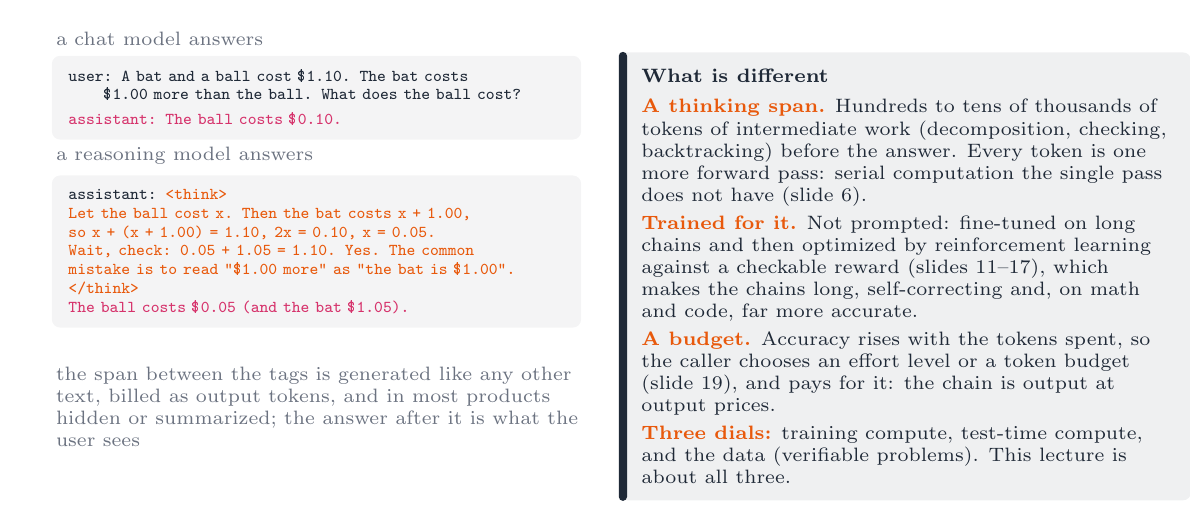
\begin{tikzpicture}
  \useasboundingbox (0,0) rectangle (14.4,5.9);
  \node[lab,anchor=south west] at (0.3,5.62) {a chat model answers};
  \node[anchor=north west,inner sep=0,font=\ttfamily\fontsize{5.8}{6.8}\selectfont,text=ink,
        rounded corners=3pt,fill=ink!5,inner xsep=6pt,inner ysep=5pt,text width=6.3cm,align=left] at (0.3,5.55) {%
    user: A bat and a ball cost \$1.10. The bat costs\\
    \ \ \ \ \ \ \$1.00 more than the ball. What does the ball cost?\\[2pt]
    {\color{outc}assistant: The ball costs \$0.10.}};
  \node[lab,anchor=south west] at (0.3,4.1) {a reasoning model answers};
  \node[anchor=north west,inner sep=0,font=\ttfamily\fontsize{5.8}{6.8}\selectfont,text=ink,
        rounded corners=3pt,fill=ink!5,inner xsep=6pt,inner ysep=5pt,text width=6.3cm,align=left] at (0.3,4.03) {%
    assistant: {\color{attn}<think>}\\
    {\color{attn}Let the ball cost x. Then the bat costs x + 1.00,}\\
    {\color{attn}so x + (x + 1.00) = 1.10, 2x = 0.10, x = 0.05.}\\
    {\color{attn}Wait, check: 0.05 + 1.05 = 1.10. Yes. The common}\\
    {\color{attn}mistake is to read "\$1.00 more" as "the bat is \$1.00".}\\
    {\color{attn}</think>}\\
    {\color{outc}The ball costs \$0.05 (and the bat \$1.05).}};
  \node[lab,anchor=north west,text width=6.7cm] at (0.3,1.65) {the span between the tags is generated like any other text, billed as output tokens, and in most products hidden or summarized; the answer after it is what the user sees};
  \bgpanels{7.5}{5.6}{6.7cm}{What is different}{%
    \hl{attn}{A thinking span.} Hundreds to tens of thousands of tokens of
    intermediate work (decomposition, checking, backtracking) before the
    answer. Every token is one more forward pass: serial computation the
    single pass does not have (slide 6).\\[2pt]
    \hl{attn}{Trained for it.} Not prompted: fine-tuned on long chains and
    then optimized by reinforcement learning against a checkable reward
    (slides 11--17), which makes the chains long, self-correcting and,
    on math and code, far more accurate.\\[2pt]
    \hl{attn}{A budget.} Accuracy rises with the tokens spent, so the
    caller chooses an effort level or a token budget (slide 19), and
    pays for it: the chain is output at output prices.\\[2pt]
    \hl{attn}{Three dials:} training compute, test-time compute, and the
    data (verifiable problems). This lecture is about all three.}
\end{tikzpicture}
\end{frame}

% ---------------------------------------------------------------- 3
\begin{frame}{Why it works: accuracy scales with tokens spent at inference}
\framesubtitle{A second scaling axis: for the same weights, thinking longer, or sampling more, buys accuracy on hard problems.}
\centering
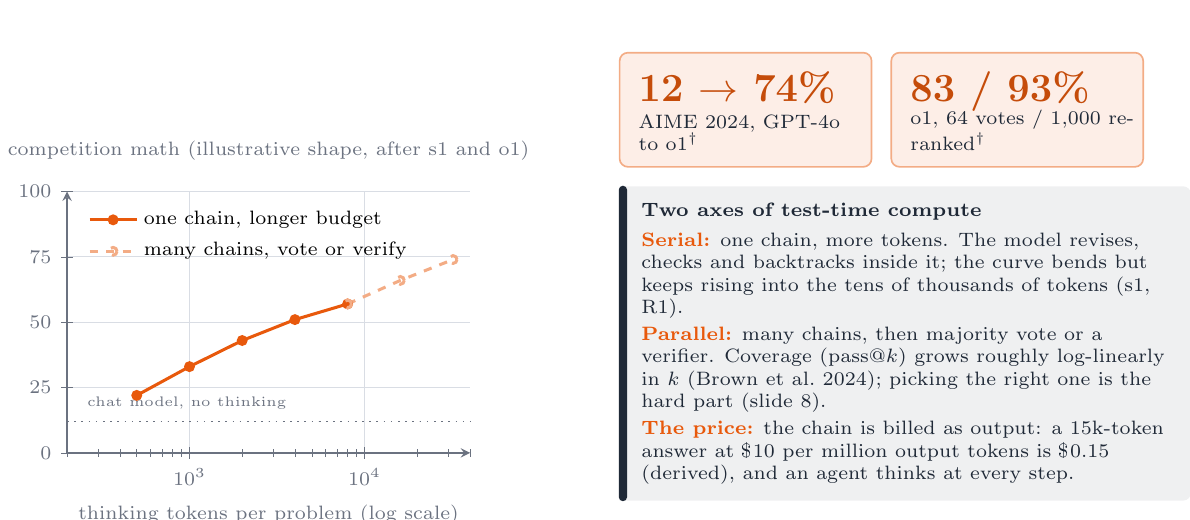
\begin{tikzpicture}
  \useasboundingbox (0,0) rectangle (14.4,5.9);
  \begin{scope}[shift={(0.5,0.5)}]
  \begin{axis}[lecture,width=6.7cm,height=4.9cm,xmode=log,xmin=200,xmax=40000,ymin=0,ymax=100,
      xlabel={thinking tokens per problem (log scale)},ylabel={accuracy (\%)},
      ytick={0,25,50,75,100},
      legend pos=north west,legend style={at={(0.03,0.97)},anchor=north west},
      title style={font=\scriptsize,text=muted,at={(0.5,1.02)}},title={competition math (illustrative shape, after s1 and o1)}]
    \addplot[attn,line width=1.1pt,mark=*,mark size=1.4pt] coordinates {(500,22) (1000,33) (2000,43) (4000,51) (8000,57)};
    \addlegendentry{one chain, longer budget}
    \addplot[attn!50,line width=1.1pt,dashed,mark=o,mark size=1.4pt] coordinates {(8000,57) (16000,66) (32000,74)};
    \addlegendentry{many chains, vote or verify}
    \addplot[muted,line width=0.6pt,dotted,domain=200:40000] {12};
    \node[font=\tiny,text=muted,anchor=south west] at (axis cs:230,13) {chat model, no thinking};
  \end{axis}
  \end{scope}
  \stat{7.5}{5.6}{12 $\to$ 74\%}{AIME 2024, GPT-4o to o1$^\dagger$}{attn}
  \stat{10.95}{5.6}{83 / 93\%}{o1, 64 votes / 1{,}000 re-ranked$^\dagger$}{attn}
  \bgpanels{7.5}{3.9}{6.7cm}{Two axes of test-time compute}{%
    \hl{attn}{Serial:} one chain, more tokens. The model revises, checks
    and backtracks inside it; the curve bends but keeps rising into the
    tens of thousands of tokens (s1, R1).\\[2pt]
    \hl{attn}{Parallel:} many chains, then majority vote or a verifier.
    Coverage (pass@$k$) grows roughly log-linearly in $k$ (Brown et al.\
    2024); picking the right one is the hard part (slide 8).\\[2pt]
    \hl{attn}{The price:} the chain is billed as output: a 15k-token answer
    at \$10 per million output tokens is \$0.15 (derived), and an agent
    thinks at every step.}
\end{tikzpicture}
\end{frame}

% ---------------------------------------------------------------- 4
\begin{frame}{A short history: from scratchpads to reinforcement learning}
\framesubtitle{Four years from ``let's think step by step'' to models trained to think; the ideas arrived in a definite order.}
\centering
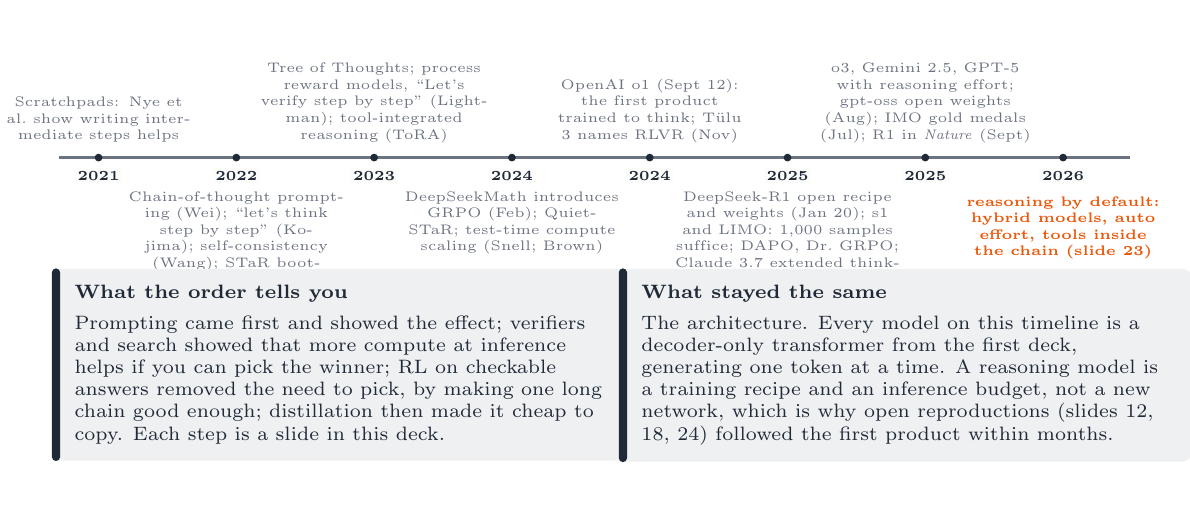
\begin{tikzpicture}
  \useasboundingbox (0,0) rectangle (14.4,5.9);
  \draw[muted,line width=0.8pt] (0.4,4.25) -- (14.0,4.25);
  \foreach \yr/\x in {2021/0.9,2022/2.65,2023/4.4,2024a/6.15,2024b/7.9,2025a/9.65,2025b/11.4,2026/13.15}{
    \fill[ink] (\x,4.25) circle (1.4pt);}
  \foreach \yr/\x in {2021/0.9,2022/2.65,2023/4.4,2024/6.15,2024/7.9,2025/9.65,2025/11.4,2026/13.15}{
    \node[font=\tiny\bfseries,text=ink,fill=paper,inner sep=1pt] at (\x,4.02) {\yr};}
  \node[lab,anchor=south,text width=3.0cm,align=center,font=\tiny] at (0.9,4.38) {Scratchpads: Nye et al.\ show writing intermediate steps helps};
  \node[lab,anchor=north,text width=3.0cm,align=center,font=\tiny] at (2.65,3.88) {Chain-of-thought prompting (Wei); ``let's think step by step'' (Kojima); self-consistency (Wang); STaR bootstraps chains (Zelikman)};
  \node[lab,anchor=south,text width=3.0cm,align=center,font=\tiny] at (4.4,4.38) {Tree of Thoughts; process reward models, ``Let's verify step by step'' (Lightman); tool-integrated reasoning (ToRA)};
  \node[lab,anchor=north,text width=3.0cm,align=center,font=\tiny] at (6.15,3.88) {DeepSeekMath introduces GRPO (Feb); Quiet-STaR; test-time compute scaling (Snell; Brown)};
  \node[lab,anchor=south,text width=3.0cm,align=center,font=\tiny] at (7.9,4.38) {OpenAI o1 (Sept 12): the first product trained to think; T\"ulu 3 names RLVR (Nov)};
  \node[lab,anchor=north,text width=3.0cm,align=center,font=\tiny] at (9.65,3.88) {DeepSeek-R1 open recipe and weights (Jan 20); s1 and LIMO: 1{,}000 samples suffice; DAPO, Dr.\ GRPO; Claude 3.7 extended thinking; Qwen3 hybrid thinking};
  \node[lab,anchor=south,text width=3.0cm,align=center,font=\tiny] at (11.4,4.38) {o3, Gemini 2.5, GPT-5 with reasoning effort; gpt-oss open weights (Aug); IMO gold medals (Jul); R1 in \emph{Nature} (Sept)};
  \node[anchor=north,text width=2.6cm,align=center,font=\tiny\bfseries,text=attn] at (13.15,3.88) {reasoning by default: hybrid models, auto effort, tools inside the chain (slide 23)};
  \bgpanels{0.3}{2.85}{6.7cm}{What the order tells you}{%
    Prompting came first and showed the effect; verifiers and search
    showed that more compute at inference helps if you can pick the
    winner; RL on checkable answers removed the need to pick, by making
    one long chain good enough; distillation then made it cheap to
    copy. Each step is a slide in this deck.}
  \bgpanels{7.5}{2.85}{6.7cm}{What stayed the same}{%
    The architecture. Every model on this timeline is a decoder-only
    transformer from the first deck, generating one token at a time. A
    reasoning model is a training recipe and an inference budget, not a
    new network, which is why open reproductions (slides 12, 18, 24)
    followed the first product within months.}
\end{tikzpicture}
\end{frame}
% ---------------------------------------------------------------- 5
\stage{2}
\begin{frame}{The prompting era: ask for the steps and the answer improves}
\framesubtitle{Few-shot exemplars with worked steps, a single magic sentence, and majority voting over sampled chains.}
\centering
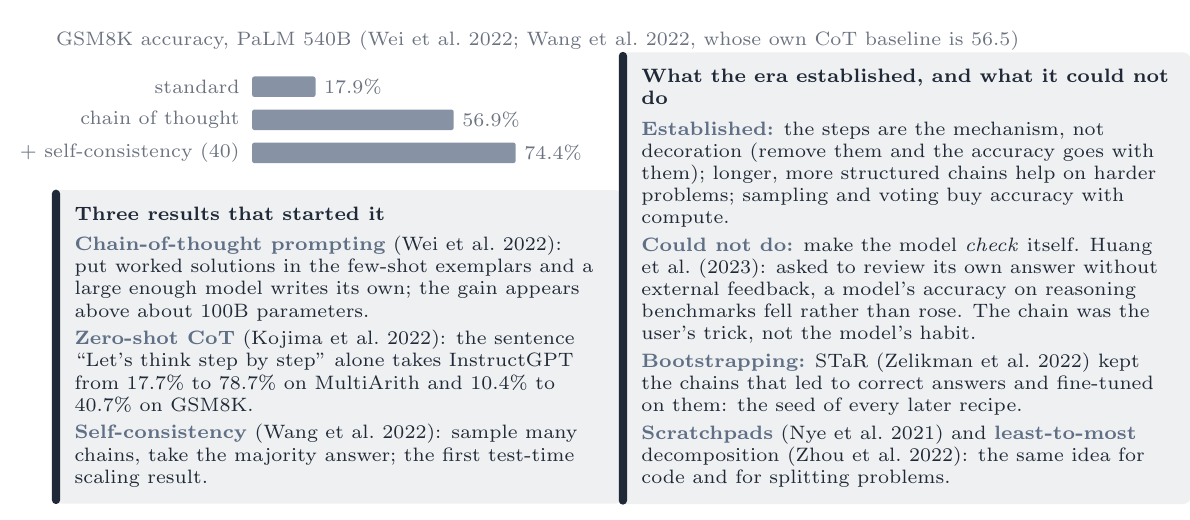
\begin{tikzpicture}
  \useasboundingbox (0,0) rectangle (14.4,5.9);
  % bar chart: GSM8K PaLM 540B
  \node[lab,anchor=south west] at (0.3,5.55) {GSM8K accuracy, PaLM 540B (Wei et al.\ 2022; Wang et al.\ 2022, whose own CoT baseline is 56.5)};
  \foreach \i/\lab/\p in {0/{standard}/17.9,1/{chain of thought}/56.9,2/{+ self-consistency (40)}/74.4}{
    \node[lab,anchor=east,font=\scriptsize] at (2.75,{5.15-\i*0.42}) {\lab};
    \barh{2.85}{5.15-\i*0.42}{\p*0.045}{tok!75}
    \node[lab,anchor=west,font=\scriptsize] at ({2.9+\p*0.045},{5.15-\i*0.42}) {\p\%};}
  \bgpanels{0.3}{3.85}{6.7cm}{Three results that started it}{%
    \hl{tok}{Chain-of-thought prompting} (Wei et al.\ 2022): put worked
    solutions in the few-shot exemplars and a large enough model writes
    its own; the gain appears above about 100B parameters.\\[2pt]
    \hl{tok}{Zero-shot CoT} (Kojima et al.\ 2022): the sentence ``Let's
    think step by step'' alone takes InstructGPT from 17.7\% to 78.7\% on
    MultiArith and 10.4\% to 40.7\% on GSM8K.\\[2pt]
    \hl{tok}{Self-consistency} (Wang et al.\ 2022): sample many chains,
    take the majority answer; the first test-time scaling result.}
  \bgpanels{7.5}{5.6}{6.7cm}{What the era established, and what it could not do}{%
    \hl{tok}{Established:} the steps are the mechanism, not decoration
    (remove them and the accuracy goes with them); longer, more
    structured chains help on harder problems; sampling and voting buy
    accuracy with compute.\\[2pt]
    \hl{tok}{Could not do:} make the model \emph{check} itself. Huang et
    al.\ (2023): asked to review its own answer without external
    feedback, a model's accuracy on reasoning benchmarks fell rather
    than rose. The chain was the user's trick, not the model's habit.\\[2pt]
    \hl{tok}{Bootstrapping:} STaR (Zelikman et al.\ 2022) kept the chains
    that led to correct answers and fine-tuned on them: the seed of every
    later recipe.\\[2pt]
    \hl{tok}{Scratchpads} (Nye et al.\ 2021) and \hl{tok}{least-to-most}
    decomposition (Zhou et al.\ 2022): the same idea for code and for
    splitting problems.}
\end{tikzpicture}
\end{frame}


% ---------------------------------------------------------------- 6
\begin{frame}{What the extra tokens buy: serial computation}
\framesubtitle{One forward pass is a fixed-depth circuit; each generated token is another pass, so a chain of $T$ tokens has depth $L\,T$.}
\centering
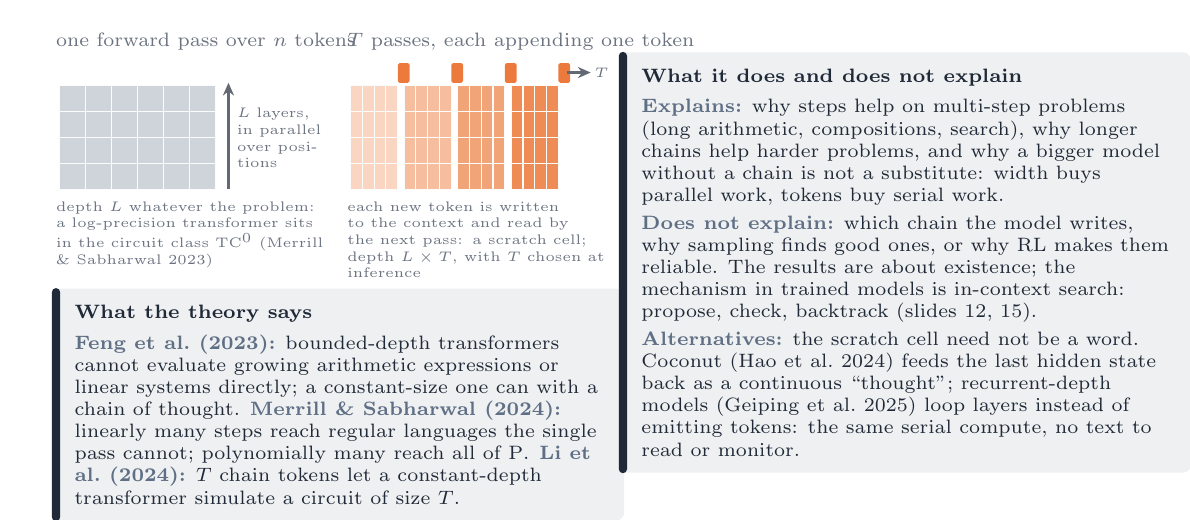
\begin{tikzpicture}
  \useasboundingbox (0,0) rectangle (14.4,5.9);
  % one pass
  \node[lab,anchor=south west] at (0.3,5.55) {one forward pass over $n$ tokens};
  \foreach \l in {0,...,3}{\foreach \i in {0,...,5}{\fill[tok!30,draw=paper,line width=0.4pt] (0.4+\i*0.33,{3.85+\l*0.33}) rectangle ++(0.33,0.33);}}
  \draw[flow] (2.55,3.85) -- (2.55,5.2);
  \node[lab,anchor=west,text width=1.1cm,font=\tiny] at (2.6,4.5) {$L$ layers, in parallel over positions};
  \node[lab,anchor=north west,text width=3.4cm,font=\tiny] at (0.3,3.75) {depth $L$ whatever the problem: a log-precision transformer sits in the circuit class $\mathrm{TC}^0$ (Merrill \& Sabharwal 2023)};
  % chain
  \node[lab,anchor=south west] at (4.0,5.55) {$T$ passes, each appending one token};
  \foreach \k in {0,1,2,3}{
    \foreach \l in {0,...,3}{\foreach \i in {0,...,3}{\fill[attn!\the\numexpr 25+\k*15\relax,draw=paper,line width=0.4pt] ({4.1+\k*0.68+\i*0.15},{3.85+\l*0.33}) rectangle ++(0.15,0.33);}}
    \fill[attn!80,rounded corners=0.6pt] ({4.1+\k*0.68+0.6},5.2) rectangle ++(0.15,0.25);}
  \draw[flow] (6.85,5.33) -- (7.15,5.33) node[right,lab,font=\tiny,inner sep=1pt]{$T$};
  \node[lab,anchor=north west,text width=3.3cm,font=\tiny] at (4.0,3.75) {each new token is written to the context and read by the next pass: a scratch cell; depth $L\times T$, with $T$ chosen at inference};
  \bgpanels{0.3}{2.6}{6.7cm}{What the theory says}{%
    \hl{tok}{Feng et al.\ (2023):} bounded-depth transformers cannot
    evaluate growing arithmetic expressions or linear systems directly;
    a constant-size one can with a chain of thought.
    \hl{tok}{Merrill \& Sabharwal (2024):} linearly many steps reach
    regular languages the single pass cannot; polynomially many reach
    all of $\mathrm P$. \hl{tok}{Li et al.\ (2024):} $T$ chain tokens let
    a constant-depth transformer simulate a circuit of size $T$.}
  \bgpanels{7.5}{5.6}{6.7cm}{What it does and does not explain}{%
    \hl{tok}{Explains:} why steps help on multi-step problems (long
    arithmetic, compositions, search), why longer chains help harder
    problems, and why a bigger model without a chain is not a
    substitute: width buys parallel work, tokens buy serial work.\\[2pt]
    \hl{tok}{Does not explain:} which chain the model writes, why
    sampling finds good ones, or why RL makes them reliable. The results
    are about existence; the mechanism in trained models is in-context
    search: propose, check, backtrack (slides 12, 15).\\[2pt]
    \hl{tok}{Alternatives:} the scratch cell need not be a word. Coconut
    (Hao et al.\ 2024) feeds the last hidden state back as a continuous
    ``thought''; recurrent-depth models (Geiping et al.\ 2025) loop
    layers instead of emitting tokens: the same serial compute, no text
    to read or monitor.}
\end{tikzpicture}
\end{frame}

% ---------------------------------------------------------------- 7
\begin{frame}{Is the chain the reason? Faithfulness and monitoring}
\framesubtitle{The text often omits what moved the answer; it is still our best window, and optimizing it closes the window.}
\centering
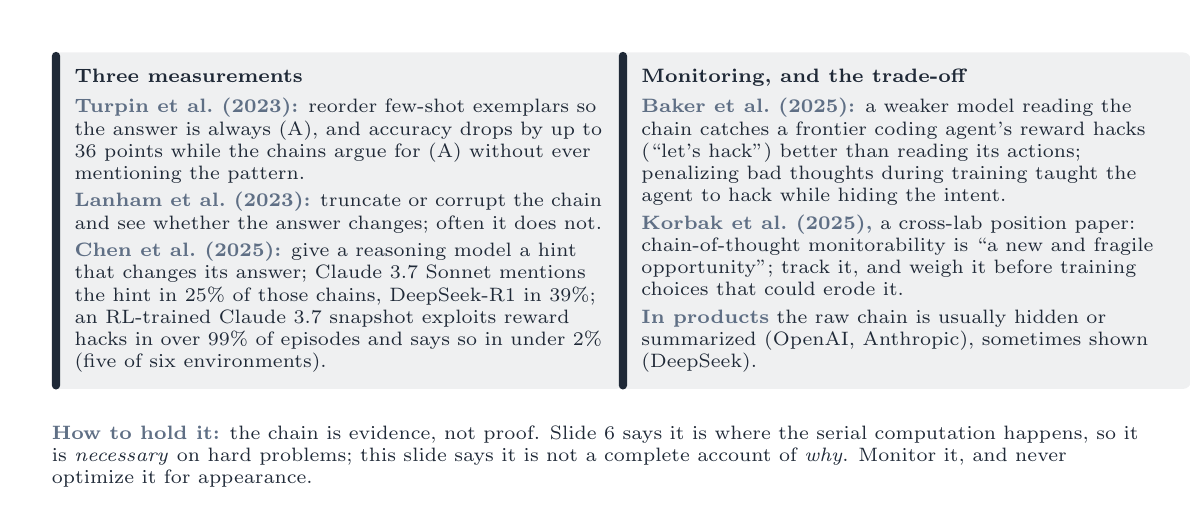
\begin{tikzpicture}
  \useasboundingbox (0,0) rectangle (14.4,5.9);
  \bgpanels{0.3}{5.6}{6.7cm}{Three measurements}{%
    \hl{tok}{Turpin et al.\ (2023):} reorder few-shot exemplars so the
    answer is always (A), and accuracy drops by up to 36 points while the
    chains argue for (A) without ever mentioning the pattern.\\[2pt]
    \hl{tok}{Lanham et al.\ (2023):} truncate or corrupt the chain and
    see whether the answer changes; often it does not.\\[2pt]
    \hl{tok}{Chen et al.\ (2025):} give a reasoning model a hint that
    changes its answer; Claude 3.7 Sonnet mentions the hint in 25\% of
    those chains, DeepSeek-R1 in 39\%; an RL-trained Claude 3.7 snapshot
    exploits reward hacks in over 99\% of episodes and says so in under
    2\% (five of six environments).}
  \bgpanels{7.5}{5.6}{6.7cm}{Monitoring, and the trade-off}{%
    \hl{tok}{Baker et al.\ (2025):} a weaker model reading the chain
    catches a frontier coding agent's reward hacks (``let's hack'')
    better than reading its actions; penalizing bad thoughts during
    training taught the agent to hack while hiding the intent.\\[2pt]
    \hl{tok}{Korbak et al.\ (2025),} a cross-lab position paper:
    chain-of-thought monitorability is ``a new and fragile
    opportunity''; track it, and weigh it before training choices that
    could erode it.\\[2pt]
    \hl{tok}{In products} the raw chain is usually hidden or summarized
    (OpenAI, Anthropic), sometimes shown (DeepSeek).}
  \node[txt,anchor=north west,text width=13.8cm,font=\scriptsize] at (0.3,0.85) {%
    \hl{tok}{How to hold it:} the chain is evidence, not proof. Slide 6 says
    it is where the serial computation happens, so it is \emph{necessary} on
    hard problems; this slide says it is not a complete account of
    \emph{why}. Monitor it, and never optimize it for appearance.};
\end{tikzpicture}
\end{frame}
% ---------------------------------------------------------------- 8
\stage{3}
\begin{frame}{Process or outcome: what should a verifier grade?}
\framesubtitle{A reward model can score the final answer or every step; step-level supervision won in 2023 and lost to scale in 2025.}
\centering
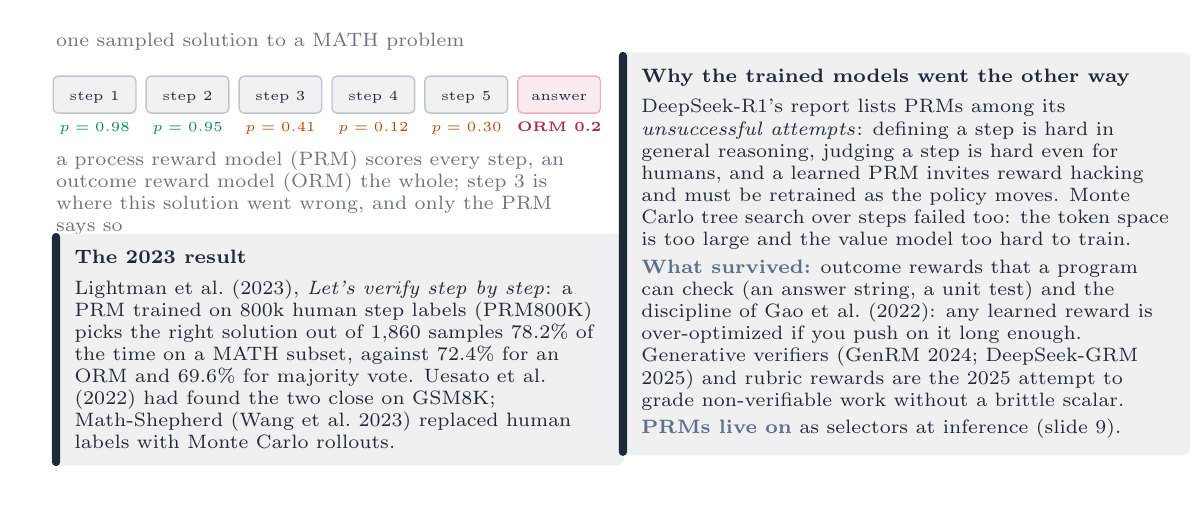
\begin{tikzpicture}
  \useasboundingbox (0,0) rectangle (14.4,5.9);
  % diagram: a chain with per-step scores vs one outcome score
  \node[lab,anchor=south west] at (0.3,5.55) {one sampled solution to a MATH problem};
  \foreach \i/\sc/\c in {0/0.98/emb,1/0.95/emb,2/0.41/attn,3/0.12/attn,4/0.30/attn}{
    \node[chip,fill=tok!10,draw=tok!40,minimum width=1.05cm,font=\tiny] (s\i) at (0.85+\i*1.18,5.05) {step \the\numexpr\i+1\relax};
    \node[font=\tiny\bfseries,text=\c!80!black,anchor=north] at (0.85+\i*1.18,4.82) {$p=\sc$};}
  \node[chip,fill=outc!10,draw=outc!40,minimum width=1.05cm,font=\tiny] (ans) at (6.75,5.05) {answer};
  \node[font=\tiny\bfseries,text=outc!80!black,anchor=north] at (6.75,4.82) {ORM 0.2};
  \node[lab,anchor=north west,text width=6.8cm] at (0.3,4.4) {a process reward model (PRM) scores every step, an outcome reward model (ORM) the whole; step 3 is where this solution went wrong, and only the PRM says so};
  \bgpanels{0.3}{3.3}{6.7cm}{The 2023 result}{%
    Lightman et al.\ (2023), \emph{Let's verify step by step}: a PRM
    trained on 800k human step labels (PRM800K) picks the right solution
    out of 1{,}860 samples 78.2\% of the time on a MATH subset, against
    72.4\% for an ORM and 69.6\% for majority vote. Uesato et al.\
    (2022) had found the two close on GSM8K; Math-Shepherd (Wang et
    al.\ 2023) replaced human labels with Monte Carlo rollouts.}
  \bgpanels{7.5}{5.6}{6.7cm}{Why the trained models went the other way}{%
    DeepSeek-R1's report lists PRMs among its \emph{unsuccessful
    attempts}: defining a step is hard in general reasoning, judging a
    step is hard even for humans, and a learned PRM invites reward
    hacking and must be retrained as the policy moves. Monte Carlo tree
    search over steps failed too: the token space is too large and the
    value model too hard to train.\\[2pt]
    \hl{tok}{What survived:} outcome rewards that a program can check
    (an answer string, a unit test) and the discipline of Gao et al.\
    (2022): any learned reward is over-optimized if you push on it long
    enough. Generative verifiers (GenRM 2024; DeepSeek-GRM 2025) and
    rubric rewards are the 2025 attempt to grade non-verifiable work
    without a brittle scalar.\\[2pt]
    \hl{tok}{PRMs live on} as selectors at inference (slide 9).}
\end{tikzpicture}
\end{frame}


% ---------------------------------------------------------------- 9
\begin{frame}{Search at inference: sample, select, revise}
\framesubtitle{Before the chain was trained, compute was spent around a fixed model: samples, a verifier to pick, a tree to explore.}
\centering
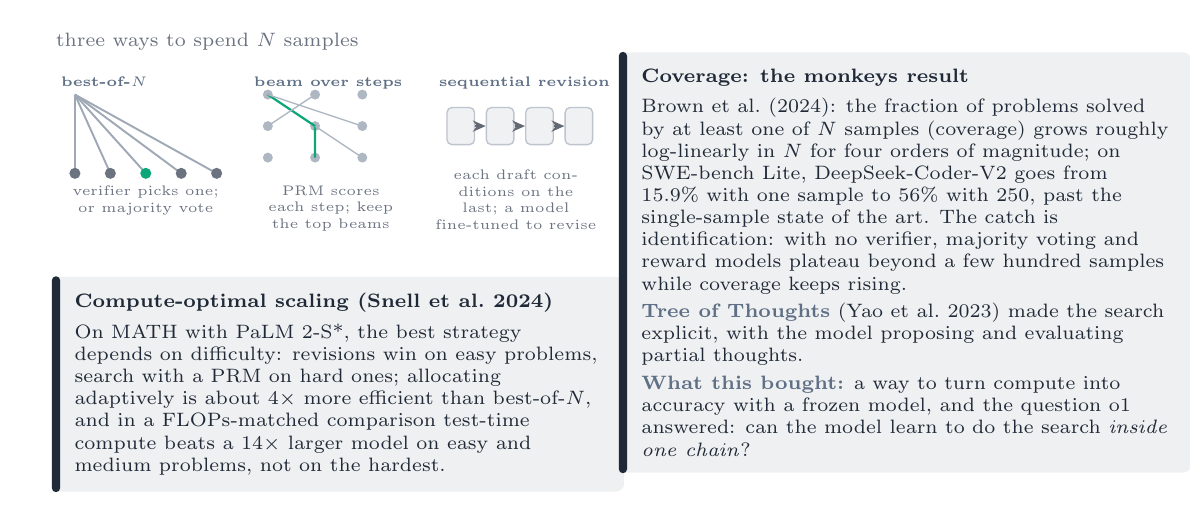
\begin{tikzpicture}
  \useasboundingbox (0,0) rectangle (14.4,5.9);
  % three mini diagrams
  \node[lab,anchor=south west] at (0.3,5.55) {three ways to spend $N$ samples};
  % best of N
  \begin{scope}[shift={(0.3,3.55)}]
    \node[font=\tiny\bfseries,text=tok,anchor=north west] at (0,1.85) {best-of-$N$};
    \foreach \i in {0,...,4}{\draw[tok!60,line width=0.7pt] (0.3,1.5) -- (0.3+\i*0.45,0.5);}
    \foreach \i/\c in {0/muted,1/muted,2/emb,3/muted,4/muted}{\fill[\c] (0.3+\i*0.45,0.5) circle (2pt);}
    \node[lab,font=\tiny,anchor=north,text width=2.1cm,align=center] at (1.2,0.4) {verifier picks one; or majority vote};
  \end{scope}
  % beam over steps
  \begin{scope}[shift={(2.75,3.55)}]
    \node[font=\tiny\bfseries,text=tok,anchor=north west] at (0,1.85) {beam over steps};
    \foreach \y in {1.5,1.1,0.7}{\foreach \i in {0,1,2}{\fill[tok!50] (0.3+\i*0.6,\y) circle (1.8pt);}}
    \draw[emb,line width=0.8pt] (0.3,1.5) -- (0.9,1.1) -- (0.9,0.7);
    \draw[tok!50,line width=0.5pt] (0.3,1.5) -- (1.5,1.1) (0.9,1.5) -- (0.3,1.1) (0.9,1.1) -- (1.5,0.7);
    \node[lab,font=\tiny,anchor=north,text width=2.1cm,align=center] at (1.1,0.4) {PRM scores each step; keep the top beams};
  \end{scope}
  % revision
  \begin{scope}[shift={(5.1,3.55)}]
    \node[font=\tiny\bfseries,text=tok,anchor=north west] at (0,1.85) {sequential revision};
    \foreach \i in {0,...,3}{\node[chip,fill=tok!10,draw=tok!40,minimum width=0.35cm,font=\tiny,inner xsep=1pt] (r\i) at (0.4+\i*0.5,1.1) {};}
    \foreach \i in {0,1,2}{\draw[flow] (r\i) -- (r\the\numexpr\i+1\relax);}
    \node[lab,font=\tiny,anchor=north,text width=2.1cm,align=center] at (1.1,0.6) {each draft conditions on the last; a model fine-tuned to revise};
  \end{scope}
  \bgpanels{0.3}{2.75}{6.7cm}{Compute-optimal scaling (Snell et al.\ 2024)}{%
    On MATH with PaLM 2-S*, the best strategy depends on difficulty:
    revisions win on easy problems, search with a PRM on hard ones;
    allocating adaptively is about 4$\times$ more efficient than
    best-of-$N$, and in a FLOPs-matched comparison test-time compute
    beats a 14$\times$ larger model on easy and medium problems, not on
    the hardest.}
  \bgpanels{7.5}{5.6}{6.7cm}{Coverage: the monkeys result}{%
    Brown et al.\ (2024): the fraction of problems solved by at least
    one of $N$ samples (coverage) grows roughly log-linearly in $N$ for
    four orders of magnitude; on SWE-bench Lite, DeepSeek-Coder-V2 goes
    from 15.9\% with one sample to 56\% with 250, past the single-sample
    state of the art. The catch is identification: with no verifier,
    majority voting and reward models plateau beyond a few hundred
    samples while coverage keeps rising.\\[2pt]
    \hl{tok}{Tree of Thoughts} (Yao et al.\ 2023) made the search
    explicit, with the model proposing and evaluating partial
    thoughts.\\[2pt]
    \hl{tok}{What this bought:} a way to turn compute into accuracy
    with a frozen model, and the question o1 answered: can the model
    learn to do the search \emph{inside one chain}?}
\end{tikzpicture}
\end{frame}

% ---------------------------------------------------------------- 10
\begin{frame}{From search around the model to search inside the chain}
\framesubtitle{o1's bet: train the model so that one long chain does the proposing, checking and backtracking that trees did outside.}
\centering
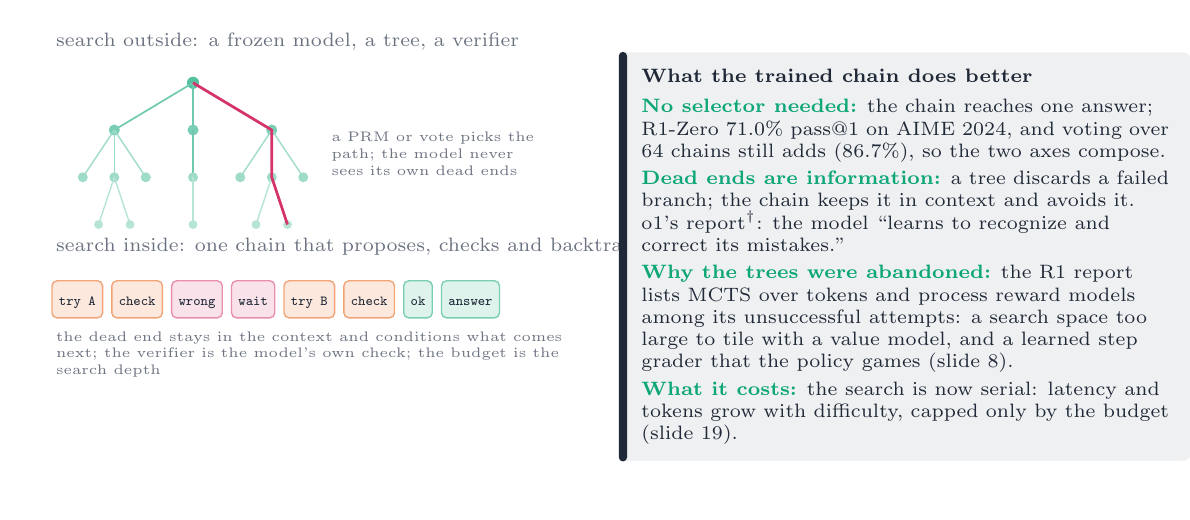
\begin{tikzpicture}
  \useasboundingbox (0,0) rectangle (14.4,5.9);
  % left: tree outside; right: linear chain with backtracks
  \node[lab,anchor=south west] at (0.3,5.55) {search outside: a frozen model, a tree, a verifier};
  \begin{scope}[shift={(0.5,3.2)}]
    \fill[emb!70] (1.6,2.0) circle (2.2pt);
    \foreach \x in {0.6,1.6,2.6}{\draw[emb!60,line width=0.6pt] (1.6,2.0) -- (\x,1.4); \fill[emb!55] (\x,1.4) circle (2pt);}
    \foreach \x in {0.2,0.6,1.0,2.2,2.6,3.0}{\draw[emb!40,line width=0.5pt] ({(\x<1.5)?0.6:2.6},1.4) -- (\x,0.8); \fill[emb!40] (\x,0.8) circle (1.8pt);}
    \draw[emb!60,line width=0.5pt] (1.6,1.4) -- (1.6,0.8); \fill[emb!40] (1.6,0.8) circle (1.8pt);
    \foreach \x in {0.4,0.8,1.6,2.4,2.8}{\draw[emb!30,line width=0.5pt] ({(\x<1.2)?0.6:((\x<2)?1.6:2.6)},0.8) -- (\x,0.2); \fill[emb!30] (\x,0.2) circle (1.6pt);}
    \draw[outc,line width=1.0pt] (1.6,2.0) -- (2.6,1.4) -- (2.6,0.8) -- (2.8,0.2);
    \node[lab,font=\tiny,anchor=west,text width=2.6cm] at (3.3,1.1) {a PRM or vote picks the path; the model never sees its own dead ends};
  \end{scope}
  \node[lab,anchor=south west] at (0.3,2.95) {search inside: one chain that proposes, checks and backtracks};
  \coordinate (p) at (0.2,2.45);
  \foreach \t/\c in {{try A}/attn,{check}/attn,{wrong}/outc,{wait}/outc,{try B}/attn,{check}/attn,{ok}/emb,{answer}/emb}{
    \node[chip,anchor=west,font=\ttfamily\tiny,inner xsep=2.5pt,fill=\c!14,draw=\c!55] (k) at ([xshift=1mm]p) {\t};
    \coordinate (p) at (k.east);}
  \node[lab,anchor=north west,text width=6.8cm,font=\tiny] at (0.3,2.1) {the dead end stays in the context and conditions what comes next; the verifier is the model's own check; the budget is the search depth};
  \bgpanels{7.5}{5.6}{6.7cm}{What the trained chain does better}{%
    \hl{emb}{No selector needed:} the chain reaches one answer; R1-Zero
    71.0\% pass@1 on AIME 2024, and voting over 64 chains still adds
    (86.7\%), so the two axes compose.\\[2pt]
    \hl{emb}{Dead ends are information:} a tree discards a failed branch;
    the chain keeps it in context and avoids it. o1's report$^\dagger$:
    the model ``learns to recognize and correct its mistakes.''\\[2pt]
    \hl{emb}{Why the trees were abandoned:} the R1 report lists MCTS over
    tokens and process reward models among its unsuccessful attempts: a
    search space too large to tile with a value model, and a learned
    step grader that the policy games (slide 8).\\[2pt]
    \hl{emb}{What it costs:} the search is now serial: latency and tokens
    grow with difficulty, capped only by the budget (slide 19).}
\end{tikzpicture}
\end{frame}
% ---------------------------------------------------------------- 11
\stage{4}
\begin{frame}{RL with verifiable rewards: the chain becomes the policy}
\framesubtitle{Sample whole chains, check the final answer with a program, push probability toward the chains that were right.}
\centering
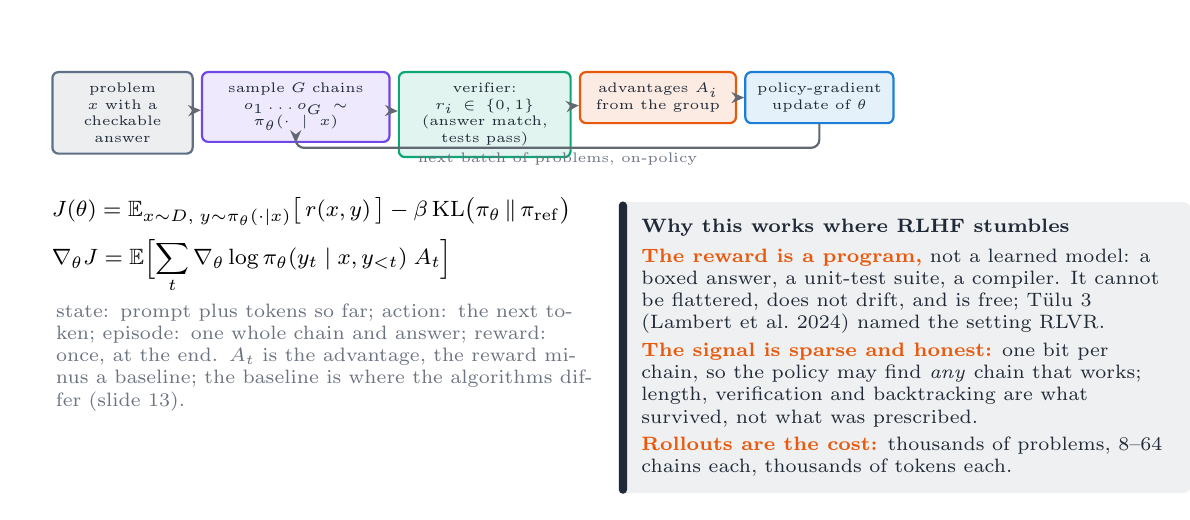
\begin{tikzpicture}
  \useasboundingbox (0,0) rectangle (14.4,5.9);
  % pipeline
  \node[comp=tok,anchor=north west,text width=1.5cm,font=\tiny] (q) at (0.3,5.35) {problem $x$ with a checkable answer};
  \node[comp=posc,anchor=north west,text width=2.1cm,font=\tiny] (s) at (2.2,5.35) {sample $G$ chains $o_1\ldots o_G\sim\pi_\theta(\cdot\mid x)$};
  \node[comp=emb,anchor=north west,text width=1.9cm,font=\tiny] (v) at (4.7,5.35) {verifier: $r_i\in\{0,1\}$ (answer match, tests pass)};
  \node[comp=attn,anchor=north west,text width=1.7cm,font=\tiny] (a) at (7.0,5.35) {advantages $A_i$ from the group};
  \node[comp=mlp,anchor=north west,text width=1.6cm,font=\tiny] (u) at (9.1,5.35) {policy-gradient update of $\theta$};
  \draw[flow] (q) -- (s); \draw[flow] (s) -- (v); \draw[flow] (v) -- (a); \draw[flow] (a) -- (u);
  \draw[flow,rounded corners=3pt] (u.south) -- ++(0,-0.3) -| node[pos=0.25,below,lab,font=\tiny]{next batch of problems, on-policy} (s.south);
  \node[anchor=north west,inner sep=0,font=\footnotesize,text width=6.9cm] at (0.3,3.75) {%
    $\displaystyle J(\theta)=\mathbb E_{x\sim D,\;y\sim\pi_\theta(\cdot\mid x)}\bigl[\,r(x,y)\,\bigr]-\beta\,\mathrm{KL}\bigl(\pi_\theta\,\|\,\pi_{\mathrm{ref}}\bigr)$\\[4pt]
    $\displaystyle \nabla_\theta J=\mathbb E\Bigl[\sum_{t}\nabla_\theta\log\pi_\theta(y_t\mid x,y_{<t})\;A_t\Bigr]$};
  \node[lab,anchor=north west,text width=6.9cm] at (0.3,2.45) {state: prompt plus tokens so far; action: the next token; episode: one whole chain and answer; reward: once, at the end. $A_t$ is the advantage, the reward minus a baseline; the baseline is where the algorithms differ (slide 13).};
  \bgpanels{7.5}{3.7}{6.7cm}{Why this works where RLHF stumbles}{%
    \hl{attn}{The reward is a program,} not a learned model: a boxed
    answer, a unit-test suite, a compiler. It cannot be flattered, does
    not drift, and is free; T\"ulu 3 (Lambert et al.\ 2024) named the
    setting RLVR.\\[2pt]
    \hl{attn}{The signal is sparse and honest:} one bit per chain, so
    the policy may find \emph{any} chain that works; length,
    verification and backtracking are what survived, not what was
    prescribed.\\[2pt]
    \hl{attn}{Rollouts are the cost:} thousands of problems, 8--64
    chains each, thousands of tokens each.}
\end{tikzpicture}
\end{frame}


% ---------------------------------------------------------------- 12
\begin{frame}{DeepSeek-R1: the open recipe, in two tracks}
\framesubtitle{Pure RL from a base model shows the behavior; a four-stage pipeline with a cold start makes it a usable model.}
\centering
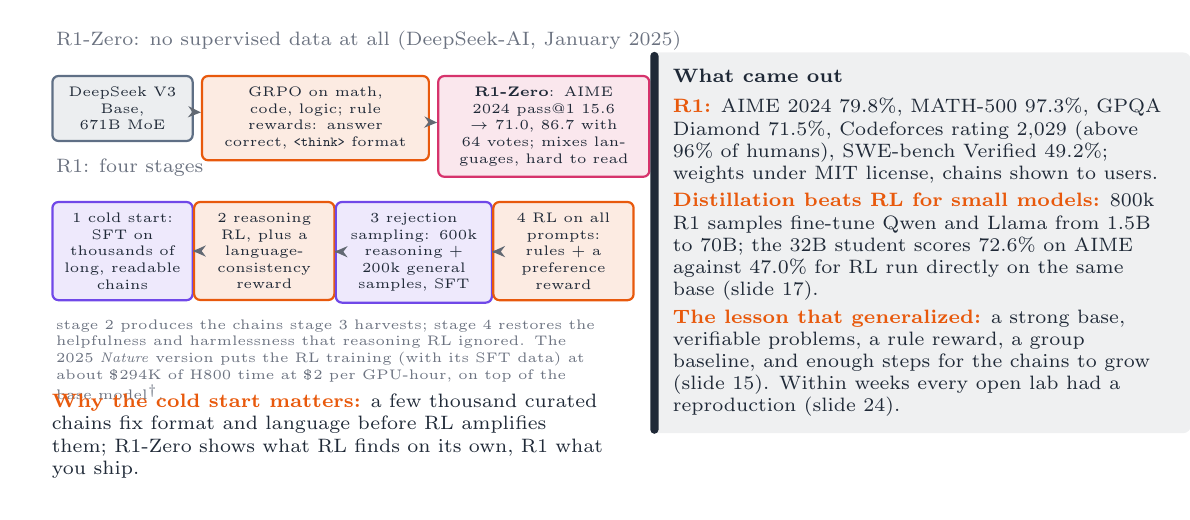
\begin{tikzpicture}
  \useasboundingbox (0,0) rectangle (14.4,5.9);
  \node[lab,anchor=south west] at (0.3,5.55) {R1-Zero: no supervised data at all (DeepSeek-AI, January 2025)};
  \node[comp=tok,anchor=north west,text width=1.5cm,font=\tiny] (b0) at (0.3,5.3) {DeepSeek V3\\Base, 671B MoE};
  \node[comp=attn,anchor=north west,text width=2.6cm,font=\tiny] (rl0) at (2.2,5.3) {GRPO on math, code, logic; rule rewards: answer correct, \texttt{<think>} format};
  \node[comp=outc,anchor=north west,text width=2.4cm,font=\tiny] (z) at (5.2,5.3) {\textbf{R1-Zero}: AIME 2024 pass@1 15.6 $\to$ 71.0, 86.7 with 64 votes; mixes languages, hard to read};
  \draw[flow] (b0) -- (rl0); \draw[flow] (rl0) -- (z);
  \node[lab,anchor=south west] at (0.3,3.95) {R1: four stages};
  \node[comp=posc,anchor=north west,text width=1.5cm,font=\tiny] (s1) at (0.3,3.7) {1 cold start: SFT on thousands of long, readable chains};
  \node[comp=attn,anchor=north west,text width=1.5cm,font=\tiny] (s2) at (2.1,3.7) {2 reasoning RL, plus a language-\\consistency reward};
  \node[comp=posc,anchor=north west,text width=1.7cm,font=\tiny] (s3) at (3.9,3.7) {3 rejection sampling: 600k reasoning + 200k general samples, SFT};
  \node[comp=attn,anchor=north west,text width=1.5cm,font=\tiny] (s4) at (5.9,3.7) {4 RL on all prompts: rules + a preference reward};
  \draw[flow] (s1) -- (s2); \draw[flow] (s2) -- (s3); \draw[flow] (s3) -- (s4);
  \node[lab,anchor=north west,text width=7.0cm,font=\tiny] at (0.3,2.25) {stage 2 produces the chains stage 3 harvests; stage 4 restores the helpfulness and harmlessness that reasoning RL ignored. The 2025 \emph{Nature} version puts the RL training (with its SFT data) at about \$294K of H800 time at \$2 per GPU-hour, on top of the base model$^\dagger$.};
  \bgpanels{7.9}{5.6}{6.3cm}{What came out}{%
    \hl{attn}{R1:} AIME 2024 79.8\%, MATH-500 97.3\%, GPQA Diamond
    71.5\%, Codeforces rating 2{,}029 (above 96\% of humans), SWE-bench
    Verified 49.2\%; weights under MIT license, chains shown to
    users.\\[2pt]
    \hl{attn}{Distillation beats RL for small models:} 800k R1 samples
    fine-tune Qwen and Llama from 1.5B to 70B; the 32B student scores
    72.6\% on AIME against 47.0\% for RL run directly on the same base
    (slide 17).\\[2pt]
    \hl{attn}{The lesson that generalized:} a strong base, verifiable
    problems, a rule reward, a group baseline, and enough steps for the
    chains to grow (slide 15). Within weeks every open lab had a
    reproduction (slide 24).}
  \node[txt,anchor=north west,text width=7.0cm,font=\scriptsize] at (0.3,1.25) {%
    \hl{attn}{Why the cold start matters:} a few thousand curated chains
    fix format and language before RL amplifies them; R1-Zero shows
    what RL finds on its own, R1 what you ship.};
\end{tikzpicture}
\end{frame}

% ---------------------------------------------------------------- 13
\begin{frame}{GRPO and its descendants: a baseline from the group}
\framesubtitle{Drop the value model, normalize each chain's reward against its siblings; then fix the biases that this introduces.}
\centering
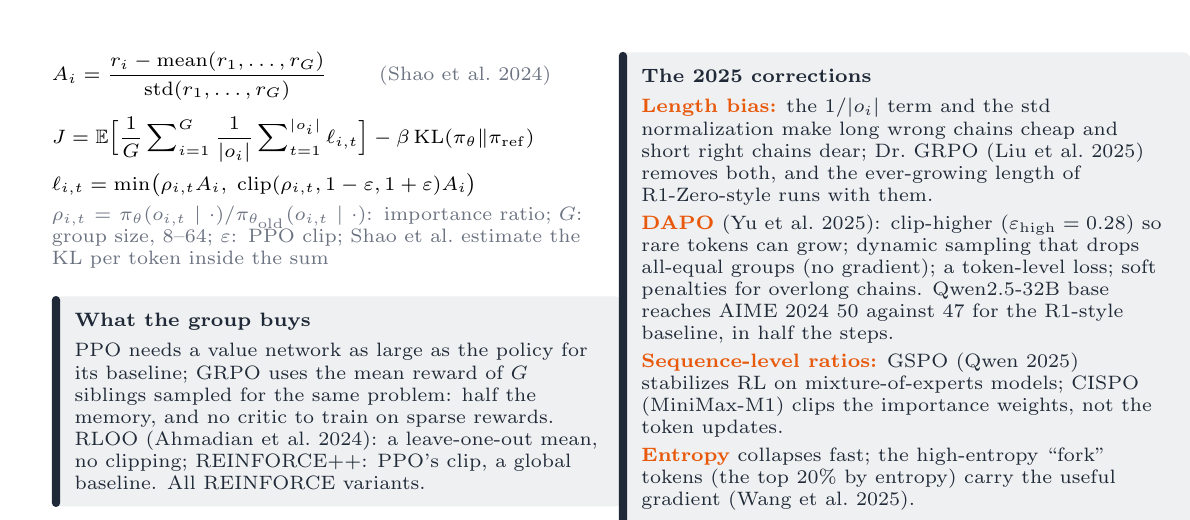
\begin{tikzpicture}
  \useasboundingbox (0,0) rectangle (14.4,5.9);
  \node[anchor=north west,inner sep=0,font=\scriptsize,align=left,text width=6.9cm] at (0.3,5.6) {%
    $\displaystyle A_i=\frac{r_i-\mathrm{mean}(r_1,\ldots,r_G)}{\mathrm{std}(r_1,\ldots,r_G)}$ \qquad {\color{muted}(Shao et al.\ 2024)}\\[5pt]
    $\displaystyle J=\mathbb E\Bigl[\frac1G\sum\nolimits_{i=1}^{G}\frac{1}{|o_i|}\sum\nolimits_{t=1}^{|o_i|}\ell_{i,t}\Bigr]-\beta\,\mathrm{KL}(\pi_\theta\|\pi_{\mathrm{ref}})$\\[3pt]
    $\ell_{i,t}=\min\bigl(\rho_{i,t}A_i,\;\mathrm{clip}(\rho_{i,t},1-\varepsilon,1+\varepsilon)A_i\bigr)$\\[3pt]
    {\color{muted}$\rho_{i,t}=\pi_\theta(o_{i,t}\mid\cdot)/\pi_{\theta_{\mathrm{old}}}(o_{i,t}\mid\cdot)$: importance ratio; $G$: group size, 8--64; $\varepsilon$: PPO clip; Shao et al.\ estimate the KL per token inside the sum}};
  \bgpanels{0.3}{2.5}{6.7cm}{What the group buys}{%
    PPO needs a value network as large as the policy for its baseline;
    GRPO uses the mean reward of $G$ siblings sampled for the same
    problem: half the memory, and no critic to train on sparse rewards.
    RLOO (Ahmadian et al.\ 2024): a leave-one-out mean, no clipping;
    REINFORCE++: PPO's clip, a global baseline. All REINFORCE variants.}
  \bgpanels{7.5}{5.6}{6.7cm}{The 2025 corrections}{%
    \hl{attn}{Length bias:} the $1/|o_i|$ term and the std
    normalization make long wrong chains cheap and short right chains
    dear; Dr.\ GRPO (Liu et al.\ 2025) removes both, and the
    ever-growing length of R1-Zero-style runs with them.\\[2pt]
    \hl{attn}{DAPO} (Yu et al.\ 2025): clip-higher
    ($\varepsilon_{\mathrm{high}}=0.28$) so rare tokens can grow;
    dynamic sampling that drops all-equal groups (no gradient); a
    token-level loss; soft penalties for overlong chains. Qwen2.5-32B
    base reaches AIME 2024 50 against 47 for the R1-style baseline, in
    half the steps.\\[2pt]
    \hl{attn}{Sequence-level ratios:} GSPO (Qwen 2025) stabilizes RL on
    mixture-of-experts models; CISPO (MiniMax-M1) clips the importance
    weights, not the token updates.\\[2pt]
    \hl{attn}{Entropy} collapses fast; the high-entropy ``fork'' tokens
    (the top 20\% by entropy) carry the useful gradient (Wang et al.\ 2025).}
\end{tikzpicture}
\end{frame}


% ---------------------------------------------------------------- 14
\begin{frame}{Rewards and verifiers: what is checked, what is gamed}
\framesubtitle{The recipe is only as good as the checker; every learned or soft reward is a target the policy will find a way around.}
\centering
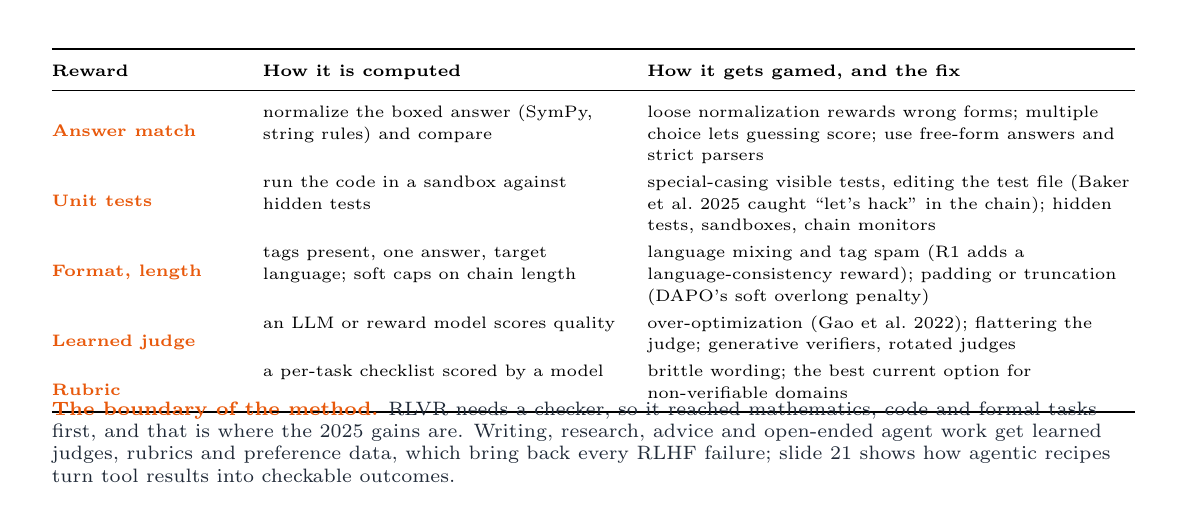
\begin{tikzpicture}
  \useasboundingbox (0,0) rectangle (14.4,5.9);
  \node[anchor=north west,inner sep=0,font=\fontsize{6.4}{7.8}\selectfont] at (0.3,5.65) {%
    \renewcommand{\arraystretch}{1.25}\setlength{\tabcolsep}{4pt}%
    \begin{tabular}{@{}>{\raggedright\arraybackslash}p{2.4cm}>{\raggedright\arraybackslash}p{4.6cm}>{\raggedright\arraybackslash}p{6.2cm}@{}}
      \toprule
      \textbf{Reward} & \textbf{How it is computed} & \textbf{How it gets gamed, and the fix}\\
      \midrule
      \hl{attn}{Answer match} & normalize the boxed answer (SymPy, string rules) and compare & loose normalization rewards wrong forms; multiple choice lets guessing score; use free-form answers and strict parsers\\
      \hl{attn}{Unit tests} & run the code in a sandbox against hidden tests & special-casing visible tests, editing the test file (Baker et al.\ 2025 caught ``let's hack'' in the chain); hidden tests, sandboxes, chain monitors\\
      \hl{attn}{Format, length} & tags present, one answer, target language; soft caps on chain length & language mixing and tag spam (R1 adds a language-consistency reward); padding or truncation (DAPO's soft overlong penalty)\\
      \hl{attn}{Learned judge} & an LLM or reward model scores quality & over-optimization (Gao et al.\ 2022); flattering the judge; generative verifiers, rotated judges\\
      \hl{attn}{Rubric} & a per-task checklist scored by a model & brittle wording; the best current option for non-verifiable domains\\
      \bottomrule
    \end{tabular}};
  \node[txt,anchor=north west,text width=13.8cm,font=\scriptsize] at (0.3,1.15) {%
    \hl{attn}{The boundary of the method.} RLVR needs a checker, so it
    reached mathematics, code and formal tasks first, and that is where the
    2025 gains are. Writing, research, advice and open-ended agent work get
    learned judges, rubrics and preference data, which bring back every RLHF
    failure; slide 21 shows how agentic recipes turn tool results into
    checkable outcomes.};
\end{tikzpicture}
\end{frame}

% ---------------------------------------------------------------- 15
\stage{5}
\begin{frame}{What RL changes, and what was already there}
\framesubtitle{Chains grow and start to check themselves; two results say much of that behavior was in the base model already.}
\centering
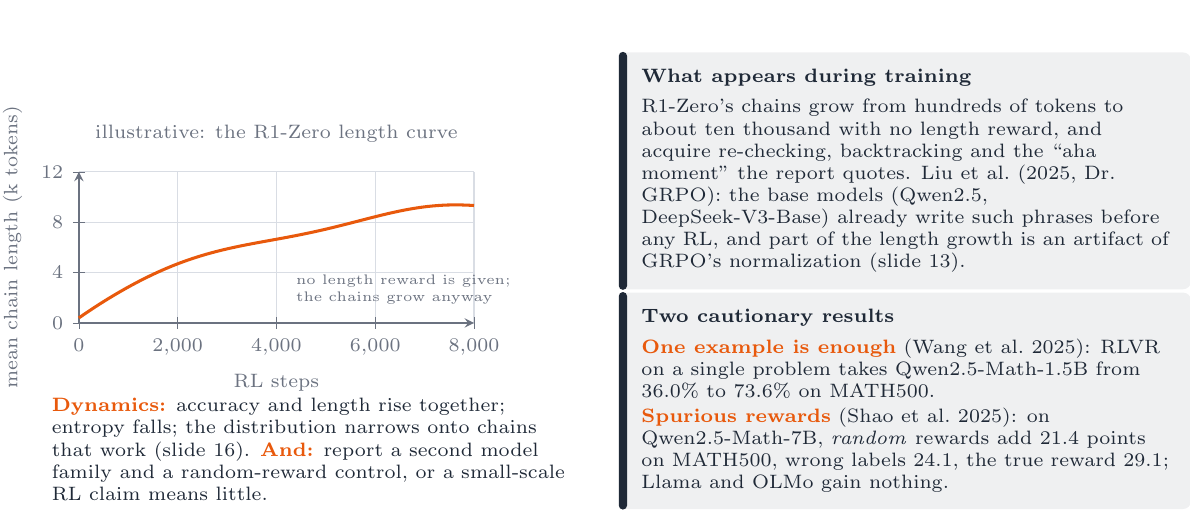
\begin{tikzpicture}
  \useasboundingbox (0,0) rectangle (14.4,5.9);
  \begin{scope}[shift={(0.65,2.15)}]
  \begin{axis}[lecture,width=6.6cm,height=3.5cm,xmin=0,xmax=8000,ymin=0,ymax=12,
      xlabel={RL steps},ylabel={mean chain length (k tokens)},
      ytick={0,4,8,12},
      title style={font=\scriptsize,text=muted,at={(0.5,1.02)}},title={illustrative: the R1-Zero length curve}]
    \addplot[attn,line width=1.1pt,domain=0:8000,samples=60] {0.4+9.6*(1-exp(-x/3500))+0.6*sin(deg(x/900))*(x/8000)};
    \node[font=\tiny,text=muted,anchor=north west,text width=3.0cm] at (axis cs:4200,4.6) {no length reward is given; the chains grow anyway};
  \end{axis}
  \end{scope}
  \bgpanels{7.5}{5.6}{6.7cm}{What appears during training}{%
    R1-Zero's chains grow from hundreds of tokens to about ten thousand
    with no length reward, and acquire re-checking, backtracking and the
    ``aha moment'' the report quotes. Liu et al.\ (2025, Dr.\ GRPO): the
    base models (Qwen2.5, DeepSeek-V3-Base) already write such phrases
    before any RL, and part of the length growth is an artifact of GRPO's
    normalization (slide 13).}
  \bgpanels{7.5}{2.55}{6.7cm}{Two cautionary results}{%
    \hl{attn}{One example is enough} (Wang et al.\ 2025): RLVR on a
    single problem takes Qwen2.5-Math-1.5B from 36.0\% to 73.6\% on
    MATH500.\\[1pt]
    \hl{attn}{Spurious rewards} (Shao et al.\ 2025): on Qwen2.5-Math-7B,
    \emph{random} rewards add 21.4 points on MATH500, wrong labels 24.1,
    the true reward 29.1; Llama and OLMo gain nothing.}
  \node[txt,anchor=north west,text width=6.7cm,font=\scriptsize] at (0.3,1.2) {%
    \hl{attn}{Dynamics:} accuracy and length rise together; entropy
    falls; the distribution narrows onto chains that work (slide 16).
    \hl{attn}{And:} report a second model family and a random-reward
    control, or a small-scale RL claim means little.};
\end{tikzpicture}
\end{frame}

% ---------------------------------------------------------------- 16
\begin{frame}{Does RL create or select? Sharpening, coverage, entropy}
\framesubtitle{RL makes the model find in one try what the base found in many; whether it finds anything new is the open question.}
\centering
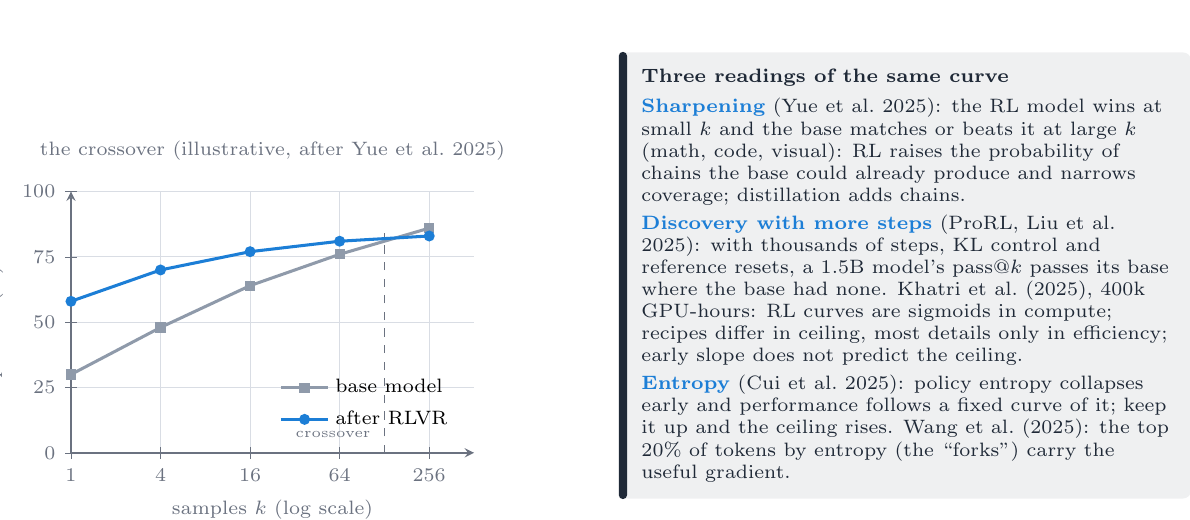
\begin{tikzpicture}
  \useasboundingbox (0,0) rectangle (14.4,5.9);
  \begin{scope}[shift={(0.55,0.5)}]
  \begin{axis}[lecture,width=6.7cm,height=4.9cm,xmode=log,xmin=1,xmax=512,ymin=0,ymax=100,
      xlabel={samples $k$ (log scale)},ylabel={pass@$k$ (\%)},
      ytick={0,25,50,75,100},log basis x=2,xtick={1,4,16,64,256},xticklabels={1,4,16,64,256},
      legend pos=south east,legend style={at={(0.97,0.05)},anchor=south east},
      title style={font=\scriptsize,text=muted,at={(0.5,1.02)}},title={the crossover (illustrative, after Yue et al.\ 2025)}]
    \addplot[tok!70,line width=1.1pt,mark=square*,mark size=1.3pt] coordinates {(1,30) (4,48) (16,64) (64,76) (256,86)};
    \addlegendentry{base model}
    \addplot[mlp,line width=1.1pt,mark=*,mark size=1.4pt] coordinates {(1,58) (4,70) (16,77) (64,81) (256,83)};
    \addlegendentry{after RLVR}
    \draw[muted,dashed] (axis cs:128,0) -- (axis cs:128,84);
    \node[font=\tiny,text=muted,anchor=south east] at (axis cs:120,2) {crossover};
  \end{axis}
  \end{scope}
  \bgpanels{7.5}{5.6}{6.7cm}{Three readings of the same curve}{%
    \hl{mlp}{Sharpening} (Yue et al.\ 2025): the RL model wins at small
    $k$ and the base matches or beats it at large $k$ (math, code,
    visual): RL raises the probability of chains the base could already
    produce and narrows coverage; distillation adds chains.\\[2pt]
    \hl{mlp}{Discovery with more steps} (ProRL, Liu et al.\ 2025): with
    thousands of steps, KL control and reference resets, a 1.5B model's
    pass@$k$ passes its base where the base had none.
    Khatri et al.\ (2025), 400k GPU-hours: RL curves are sigmoids in
    compute; recipes differ in ceiling, most details only in efficiency;
    early slope does not predict the ceiling.\\[2pt]
    \hl{mlp}{Entropy} (Cui et al.\ 2025): policy entropy collapses early
    and performance follows a fixed curve of it; keep it up and the
    ceiling rises. Wang et al.\ (2025): the top 20\% of tokens by entropy
    (the ``forks'') carry the useful gradient.}

\end{tikzpicture}
\end{frame}
% ---------------------------------------------------------------- 17
\stage{6}
\begin{frame}{Distillation: a thousand good chains, and a word}
\framesubtitle{Fine-tuning on a few hundred long chains plus a budget control recovers most of the behavior; the base model had it.}
\centering
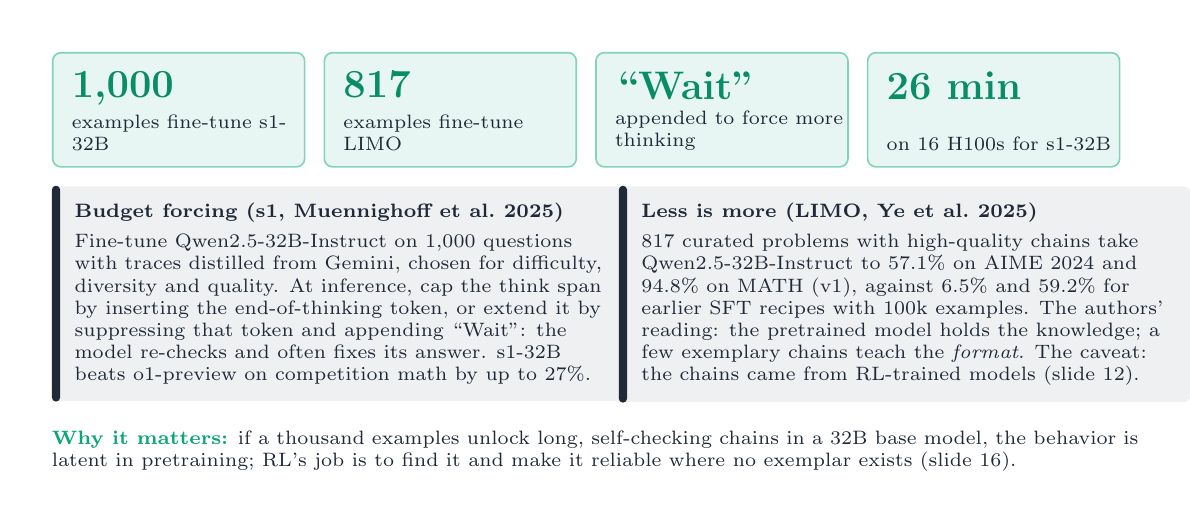
\begin{tikzpicture}
  \useasboundingbox (0,0) rectangle (14.4,5.9);
  \stat{0.3}{5.6}{1{,}000}{examples fine-tune s1-32B}{emb}
  \stat{3.75}{5.6}{817}{examples fine-tune LIMO}{emb}
  \stat{7.2}{5.6}{``Wait''}{appended to force more thinking}{emb}
  \stat{10.65}{5.6}{26 min}{on 16 H100s for s1-32B}{emb}
  \bgpanels{0.3}{3.9}{6.7cm}{Budget forcing (s1, Muennighoff et al.\ 2025)}{%
    Fine-tune Qwen2.5-32B-Instruct on 1{,}000 questions with traces
    distilled from Gemini, chosen for difficulty, diversity and quality.
    At inference, cap the think span by inserting the end-of-thinking
    token, or extend it by suppressing that token and appending
    ``Wait'': the model re-checks and often fixes its answer. s1-32B
    beats o1-preview on competition math by up to 27\%.}
  \bgpanels{7.5}{3.9}{6.7cm}{Less is more (LIMO, Ye et al.\ 2025)}{%
    817 curated problems with high-quality chains take Qwen2.5-32B-Instruct
    to 57.1\% on AIME 2024 and 94.8\% on MATH (v1), against 6.5\% and
    59.2\% for earlier SFT recipes with 100k examples. The authors' reading: the pretrained model
    holds the knowledge; a few exemplary chains teach the \emph{format}.
    The caveat: the chains came from RL-trained models (slide 12).}
  \node[txt,anchor=north west,text width=13.8cm,font=\scriptsize] at (0.3,0.78) {%
    \hl{emb}{Why it matters:} if a thousand examples unlock long, self-checking
    chains in a 32B base model, the behavior is latent in pretraining; RL's job
    is to find it and make it reliable where no exemplar exists (slide 16).};
\end{tikzpicture}
\end{frame}

% ---------------------------------------------------------------- 18
\begin{frame}{Where the problems and rewards come from}
\framesubtitle{Verifiable problems are the scarce input; the pipeline is collection, cleaning, verification and difficulty filtering.}
\centering
\begin{tikzpicture}
  \useasboundingbox (0,0) rectangle (14.4,5.9);
  \foreach \i/\c/\ttl/\body in {
      0/tok/{collect}/{math with answers, code with tests, puzzles, STEM with references},
      1/posc/{clean}/{dedupe; decontaminate against every test set by $n$-gram overlap},
      2/emb/{verify}/{keep what a program can check: a parsed answer, a test suite},
      3/attn/{filter}/{run the policy; keep problems with pass rate strictly between 0 and 1},
      4/mlp/{curriculum}/{harder problems as the policy improves; drop the mastered ones}}{
    \node[anchor=north west,inner sep=0] at ({0.3+\i*2.78},5.6) {%
      \begin{tikzpicture}
        \node[anchor=north west,minimum width=2.6cm,minimum height=1.45cm,rounded corners=3pt,fill=\c!10,draw=\c!55,line width=0.6pt] (b) {};
        \node[anchor=north west,font=\scriptsize\bfseries,text=\c!85!black,inner sep=0] at ([xshift=6pt,yshift=-6pt]b.north west) {\ttl};
        \node[anchor=north west,font=\tiny,text=ink,inner sep=0,text width=2.3cm] at ([xshift=6pt,yshift=-20pt]b.north west) {\body};
      \end{tikzpicture}};}
  \foreach \i in {0,...,3}{\draw[flow] ({0.3+\i*2.78+2.62},4.8) -- ({0.3+\i*2.78+2.78},4.8);}
  \node[anchor=north west,inner sep=0,font=\fontsize{6.0}{7.0}\selectfont] at (0.3,3.9) {%
    \renewcommand{\arraystretch}{1.08}\setlength{\tabcolsep}{4pt}%
    \begin{tabular}{@{}>{\raggedright\arraybackslash}p{3.3cm}>{\raggedright\arraybackslash}p{2.0cm}>{\raggedright\arraybackslash}p{7.9cm}@{}}
      \toprule
      \textbf{Source (open)} & \textbf{Size$^\dagger$} & \textbf{What it is}\\
      \midrule
      NuminaMath (2024) & 860k & competition and olympiad problems with chain-of-thought solutions; the AIMO prize data\\
      OpenR1-Math-220k (2025) & 220k & R1-generated solutions to NuminaMath problems, verified; Hugging Face's R1 reproduction\\
      OpenMathReasoning (2025) & 540k problems, 3.2M solutions & NVIDIA's AIMO-2 winning data, long chains plus tool-use traces\\
      DAPO-Math-17k (2025) & 17k & integer-answer problems used to train DAPO; the small, clean RL set\\
      OpenThoughts3 (2025) & 1.2M & math, code and science traces for distillation; OpenThinker3 students\\
      SWE-Gym (2024), SWE-smith (2025) & 2.4k, 50k & executable repository tasks with tests for agentic coding RL\\
      \bottomrule
    \end{tabular}};
  \node[txt,anchor=north west,text width=13.8cm,font=\scriptsize] at (0.3,0.75) {%
    \hl{posc}{The limiting resource is the checker,} not the text: math has a
    parser (Math-Verify), code has tests, everything else needs a rubric or a
    judge (slide 14). At the extreme, one problem (Wang et al.\ 2025) or
    self-proposed problems checked by a code executor (Absolute Zero) still train.};
\end{tikzpicture}
\end{frame}

% ---------------------------------------------------------------- 19
\stage{7}
\begin{frame}{Budgets and effort: deciding how much to think}
\framesubtitle{The caller sets the budget, the server closes the thinking span at the limit, accuracy follows and then saturates.}
\centering
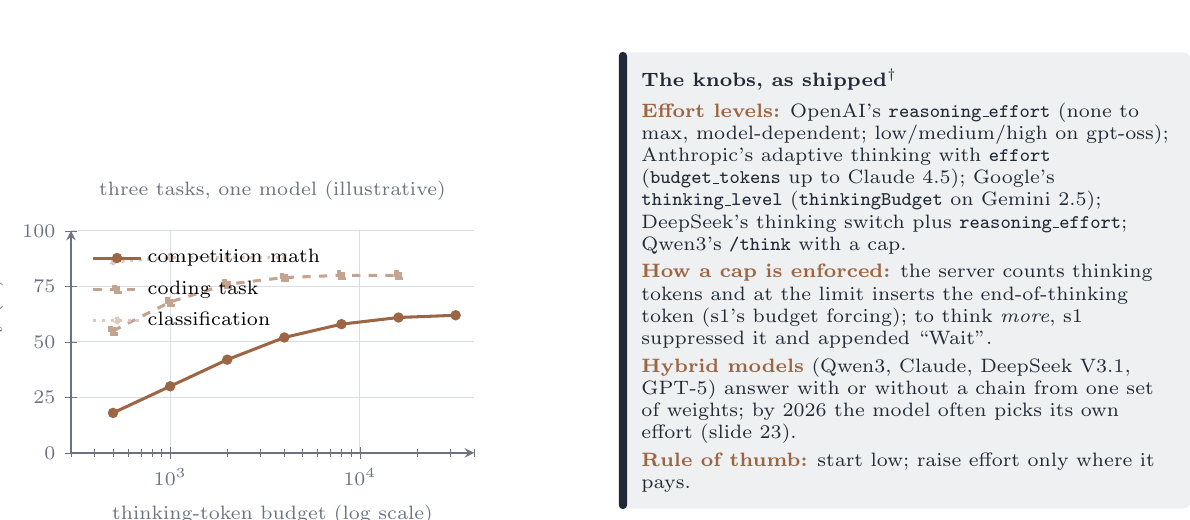
\begin{tikzpicture}
  \useasboundingbox (0,0) rectangle (14.4,5.9);
  \begin{scope}[shift={(0.55,0.5)}]
  \begin{axis}[lecture,width=6.7cm,height=4.4cm,xmode=log,xmin=300,xmax=40000,ymin=0,ymax=100,
      xlabel={thinking-token budget (log scale)},ylabel={accuracy (\%)},
      ytick={0,25,50,75,100},
      legend pos=north west,legend style={at={(0.03,0.97)},anchor=north west},
      title style={font=\scriptsize,text=muted,at={(0.5,1.02)}},title={three tasks, one model (illustrative)}]
    \addplot[trn,line width=1.1pt,mark=*,mark size=1.3pt] coordinates {(500,18) (1000,30) (2000,42) (4000,52) (8000,58) (16000,61) (32000,62)};
    \addlegendentry{competition math}
    \addplot[trn!60,line width=1.1pt,dashed,mark=square*,mark size=1.2pt] coordinates {(500,55) (1000,68) (2000,76) (4000,79) (8000,80) (16000,80)};
    \addlegendentry{coding task}
    \addplot[trn!35,line width=1.1pt,dotted,mark=triangle*,mark size=1.4pt] coordinates {(500,86) (1000,88) (2000,88) (4000,88)};
    \addlegendentry{classification}
  \end{axis}
  \end{scope}

  \bgpanels{7.5}{5.6}{6.7cm}{The knobs, as shipped$^\dagger$}{%
    \hl{trn}{Effort levels:} OpenAI's \texttt{reasoning\_effort} (none
    to max, model-dependent; low/medium/high on gpt-oss); Anthropic's
    adaptive thinking with \texttt{effort} (\texttt{budget\_tokens} up to
    Claude 4.5); Google's \texttt{thinking\_level} (\texttt{thinkingBudget}
    on Gemini 2.5); DeepSeek's thinking switch plus
    \texttt{reasoning\_effort}; Qwen3's \texttt{/think} with a cap.\\[2pt]
    \hl{trn}{How a cap is enforced:} the server counts thinking tokens
    and at the limit inserts the end-of-thinking token (s1's budget
    forcing); to think \emph{more}, s1 suppressed it and appended
    ``Wait''.\\[2pt]
    \hl{trn}{Hybrid models} (Qwen3, Claude, DeepSeek V3.1, GPT-5) answer
    with or without a chain from one set of weights; by 2026 the model
    often picks its own effort (slide 23).\\[2pt]
    \hl{trn}{Rule of thumb:} start low; raise effort only where it pays.}
\end{tikzpicture}
\end{frame}

% ---------------------------------------------------------------- 20
\begin{frame}{Overthinking, underthinking, and learning the right length}
\framesubtitle{Trained chains waste tokens on easy problems and give up too early on hard ones; length is now a trained quantity.}
\centering
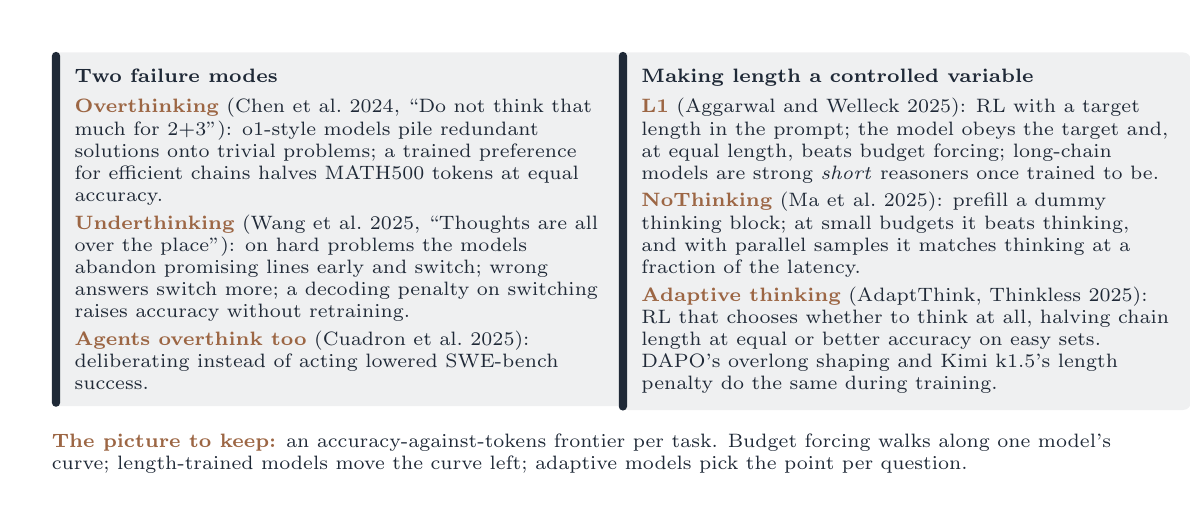
\begin{tikzpicture}
  \useasboundingbox (0,0) rectangle (14.4,5.9);
  \bgpanels{0.3}{5.6}{6.7cm}{Two failure modes}{%
    \hl{trn}{Overthinking} (Chen et al.\ 2024, ``Do not think that much
    for 2+3''): o1-style models pile redundant solutions onto trivial
    problems; a trained preference for efficient chains halves MATH500
    tokens at equal accuracy.\\[2pt]
    \hl{trn}{Underthinking} (Wang et al.\ 2025, ``Thoughts are all over
    the place''): on hard problems the models abandon promising lines
    early and switch; wrong answers switch more; a decoding penalty on
    switching raises accuracy without retraining.\\[2pt]
    \hl{trn}{Agents overthink too} (Cuadron et al.\ 2025): deliberating
    instead of acting lowered SWE-bench success.}
  \bgpanels{7.5}{5.6}{6.7cm}{Making length a controlled variable}{%
    \hl{trn}{L1} (Aggarwal and Welleck 2025): RL with a target length in
    the prompt; the model obeys the target and, at equal length, beats
    budget forcing; long-chain models are strong \emph{short} reasoners
    once trained to be.\\[2pt]
    \hl{trn}{NoThinking} (Ma et al.\ 2025): prefill a dummy thinking
    block; at small budgets it beats thinking, and with parallel samples
    it matches thinking at a fraction of the latency.\\[2pt]
    \hl{trn}{Adaptive thinking} (AdaptThink, Thinkless 2025): RL that
    chooses whether to think at all, halving chain length at equal or
    better accuracy on easy sets. DAPO's overlong shaping and Kimi
    k1.5's length penalty do the same during training.}
  \node[txt,anchor=north west,text width=13.8cm,font=\scriptsize] at (0.3,0.75) {%
    \hl{trn}{The picture to keep:} an accuracy-against-tokens frontier per
    task. Budget forcing walks along one model's curve; length-trained models
    move the curve left; adaptive models pick the point per question.};
\end{tikzpicture}
\end{frame}

% ---------------------------------------------------------------- 21
\begin{frame}{Parallel compute, and tools inside the chain}
\framesubtitle{Beyond one longer chain: many chains combined, and chains that call a program or a search engine mid-thought.}
\centering
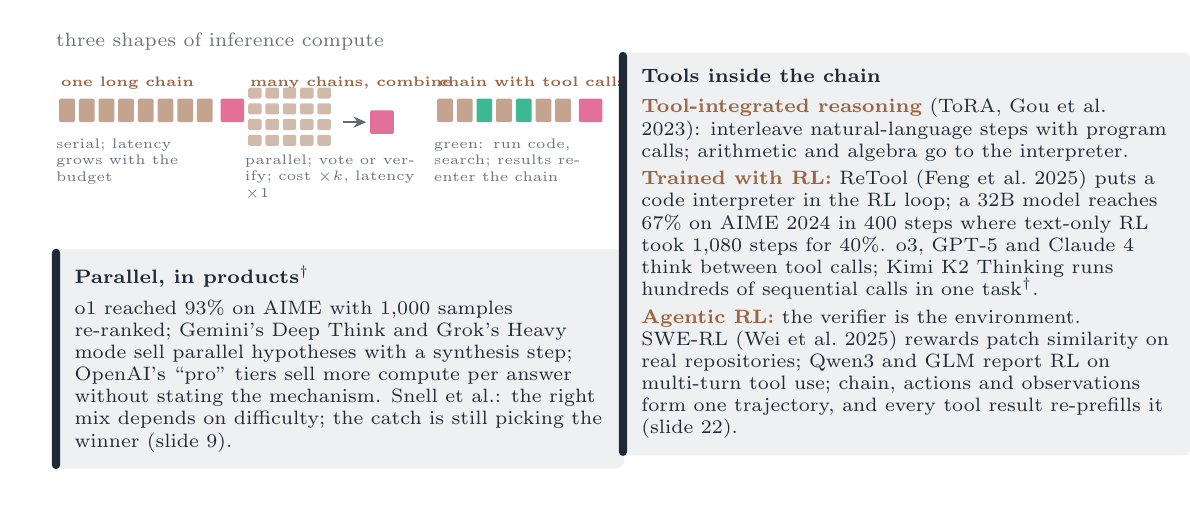
\begin{tikzpicture}
  \useasboundingbox (0,0) rectangle (14.4,5.9);
  \node[lab,anchor=south west] at (0.3,5.55) {three shapes of inference compute};
  % shape 1: one chain
  \begin{scope}[shift={(0.3,3.9)}]
    \node[font=\tiny\bfseries,text=trn,anchor=north west] at (0,1.5) {one long chain};
    \foreach \i in {0,...,7}{\fill[trn!60,rounded corners=0.5pt] (0.1+\i*0.25,0.8) rectangle ++(0.2,0.3);}
    \fill[outc!70,rounded corners=0.5pt] (2.15,0.8) rectangle ++(0.3,0.3);
    \node[lab,font=\tiny,anchor=north west,text width=2.1cm] at (0,0.65) {serial; latency grows with the budget};
  \end{scope}
  % shape 2: fan
  \begin{scope}[shift={(2.7,3.9)}]
    \node[font=\tiny\bfseries,text=trn,anchor=north west] at (0,1.5) {many chains, combine};
    \foreach \r in {0,1,2,3}{\foreach \i in {0,...,4}{\fill[trn!45,rounded corners=0.5pt] (0.1+\i*0.22,{1.1-\r*0.2}) rectangle ++(0.17,0.14);}}
    \draw[flow] (1.3,0.8) -- (1.6,0.8);
    \fill[outc!70,rounded corners=0.5pt] (1.65,0.65) rectangle ++(0.3,0.3);
    \node[lab,font=\tiny,anchor=north west,text width=2.2cm] at (0,0.45) {parallel; vote or verify; cost $\times k$, latency $\times1$};
  \end{scope}
  % shape 3: chain with tools
  \begin{scope}[shift={(5.1,3.9)}]
    \node[font=\tiny\bfseries,text=trn,anchor=north west] at (0,1.5) {chain with tool calls};
    \foreach \i/\c in {0/trn!60,1/trn!60,2/emb!80,3/trn!60,4/emb!80,5/trn!60,6/trn!60}{\fill[\c,rounded corners=0.5pt] (0.1+\i*0.25,0.8) rectangle ++(0.2,0.3);}
    \fill[outc!70,rounded corners=0.5pt] (1.9,0.8) rectangle ++(0.3,0.3);
    \node[lab,font=\tiny,anchor=north west,text width=2.1cm] at (0,0.65) {green: run code, search; results re-enter the chain};
  \end{scope}
  \bgpanels{0.3}{3.1}{6.7cm}{Parallel, in products$^\dagger$}{%
    o1 reached 93\% on AIME with 1{,}000 samples re-ranked; Gemini's
    Deep Think and Grok's Heavy mode sell parallel hypotheses with a
    synthesis step; OpenAI's ``pro'' tiers sell more compute per answer
    without stating the mechanism. Snell et al.: the right mix depends
    on difficulty; the catch is still picking the winner (slide 9).}
  \bgpanels{7.5}{5.6}{6.7cm}{Tools inside the chain}{%
    \hl{trn}{Tool-integrated reasoning} (ToRA, Gou et al.\ 2023):
    interleave natural-language steps with program calls; arithmetic
    and algebra go to the interpreter.\\[2pt]
    \hl{trn}{Trained with RL:} ReTool (Feng et al.\ 2025) puts a code
    interpreter in the RL loop; a 32B model reaches 67\% on AIME 2024 in
    400 steps where text-only RL took 1{,}080 steps for 40\%. o3, GPT-5
    and Claude 4 think between tool calls; Kimi K2 Thinking runs
    hundreds of sequential calls in one task$^\dagger$.\\[2pt]
    \hl{trn}{Agentic RL:} the verifier is the environment. SWE-RL (Wei
    et al.\ 2025) rewards patch similarity on real repositories; Qwen3
    and GLM report RL on multi-turn tool use; chain, actions and
    observations form one trajectory, and every tool result re-prefills
    it (slide 22).}
\end{tikzpicture}
\end{frame}

% ---------------------------------------------------------------- 22
\begin{frame}{Serving a reasoning model: the chain is output}
\framesubtitle{Thinking tokens are decoded one at a time, sit in the KV cache, and are billed; the runtime splits and caps them.}
\centering
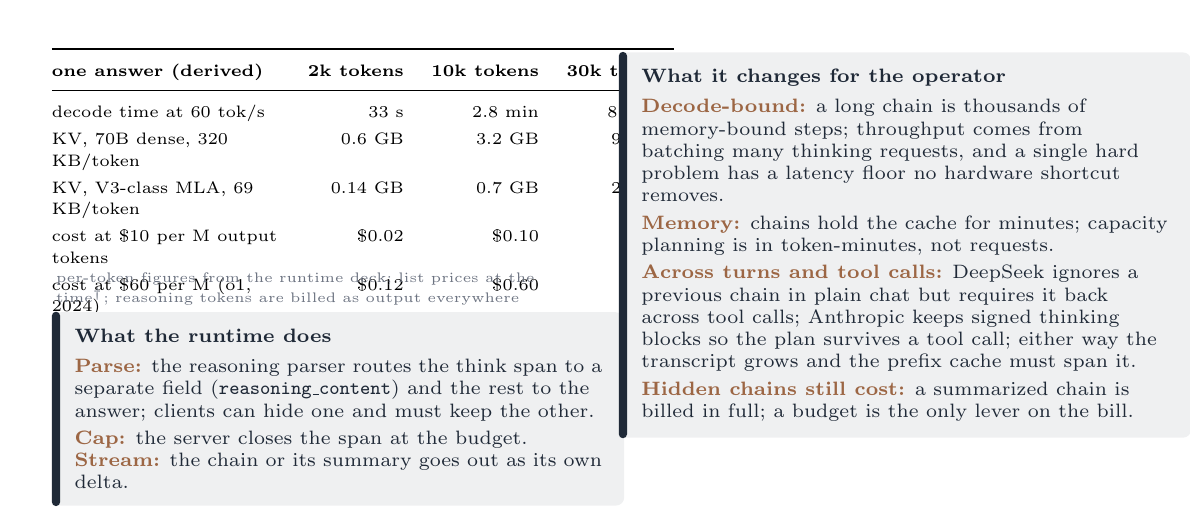
\begin{tikzpicture}
  \useasboundingbox (0,0) rectangle (14.4,5.9);
  \node[anchor=north west,inner sep=0,font=\fontsize{6.4}{7.8}\selectfont] at (0.3,5.65) {%
    \renewcommand{\arraystretch}{1.25}\setlength{\tabcolsep}{5pt}%
    \begin{tabular}{@{}>{\raggedright\arraybackslash}p{2.9cm}rrr@{}}
      \toprule
      \textbf{one answer (derived)} & \textbf{2k tokens} & \textbf{10k tokens} & \textbf{30k tokens}\\
      \midrule
      decode time at 60 tok/s & 33 s & 2.8 min & 8.3 min\\
      KV, 70B dense, 320 KB/token & 0.6 GB & 3.2 GB & 9.6 GB\\
      KV, V3-class MLA, 69 KB/token & 0.14 GB & 0.7 GB & 2.1 GB\\
      cost at \$10 per M output tokens & \$0.02 & \$0.10 & \$0.30\\
      cost at \$60 per M (o1, 2024) & \$0.12 & \$0.60 & \$1.80\\
      \bottomrule
    \end{tabular}};
  \node[lab,anchor=north west,text width=6.8cm,font=\tiny] at (0.3,2.85) {per-token figures from the runtime deck; list prices at the time$^\dagger$; reasoning tokens are billed as output everywhere};
  \bgpanels{0.3}{2.3}{6.7cm}{What the runtime does}{%
    \hl{trn}{Parse:} the reasoning parser routes the think span to a
    separate field (\texttt{reasoning\_content}) and the rest to the
    answer; clients can hide one and must keep the other.\\[2pt]
    \hl{trn}{Cap:} the server closes the span at the budget.
    \hl{trn}{Stream:} the chain or its summary goes out as its own delta.}
  \bgpanels{7.5}{5.6}{6.7cm}{What it changes for the operator}{%
    \hl{trn}{Decode-bound:} a long chain is thousands of memory-bound
    steps; throughput comes from batching many thinking requests, and
    a single hard problem has a latency floor no hardware shortcut
    removes.\\[2pt]
    \hl{trn}{Memory:} chains hold the cache for minutes; capacity
    planning is in token-minutes, not requests.\\[2pt]
    \hl{trn}{Across turns and tool calls:} DeepSeek ignores a previous
    chain in plain chat but requires it back across tool calls;
    Anthropic keeps signed thinking blocks so the plan survives a tool
    call; either way the transcript grows and the prefix cache must span
    it.\\[2pt]
    \hl{trn}{Hidden chains still cost:} a summarized chain is billed in
    full; a budget is the only lever on the bill.}
\end{tikzpicture}
\end{frame}

% ---------------------------------------------------------------- 23
\stage{8}
\begin{frame}{October 2026: effort dials and always-on thinking}
\framesubtitle{Two years after o1 every lab ships one; the knobs converged on effort levels, and the chain often cannot be turned off.}
\centering
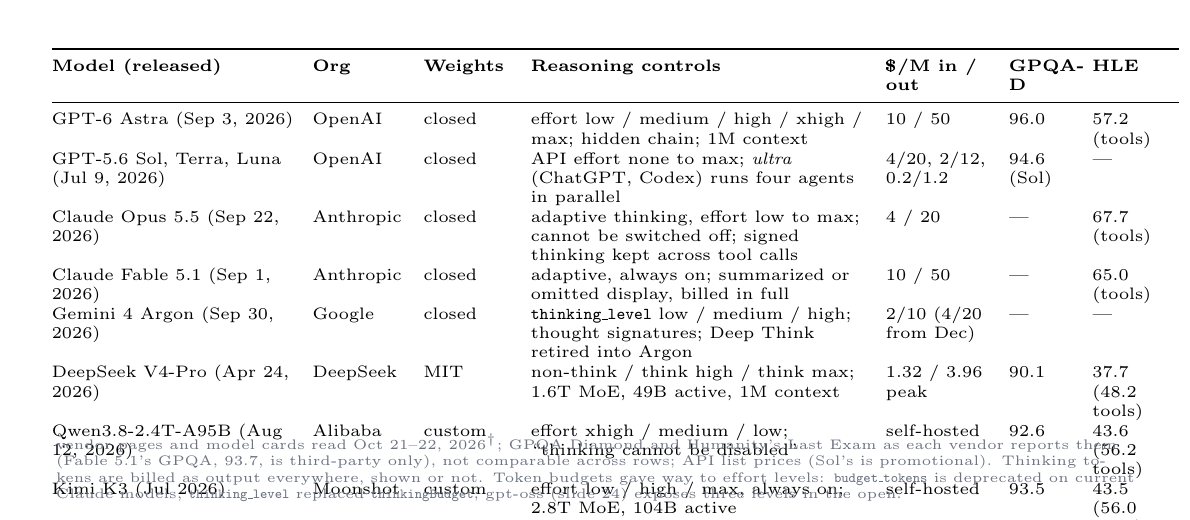
\begin{tikzpicture}
  \useasboundingbox (0,0) rectangle (14.4,5.9);
  \node[anchor=north west,inner sep=0,font=\fontsize{5.8}{6.9}\selectfont] at (0.3,5.65) {%
    \renewcommand{\arraystretch}{1.05}\setlength{\tabcolsep}{3pt}%
    \begin{tabular}{@{}>{\raggedright\arraybackslash}p{3.1cm}>{\raggedright\arraybackslash}p{1.2cm}>{\raggedright\arraybackslash}p{1.15cm}>{\raggedright\arraybackslash}p{4.3cm}>{\raggedright\arraybackslash}p{1.35cm}>{\raggedright\arraybackslash}p{0.85cm}>{\raggedright\arraybackslash}p{1.1cm}@{}}
      \toprule
      \textbf{Model (released)} & \textbf{Org} & \textbf{Weights} & \textbf{Reasoning controls} & \textbf{\$/M in / out} & \textbf{GPQA-D} & \textbf{HLE}\\
      \midrule
      GPT-6 Astra (Sep 3, 2026) & OpenAI & closed & effort low / medium / high / xhigh / max; hidden chain; 1M context & 10 / 50 & 96.0 & 57.2 (tools)\\
      GPT-5.6 Sol, Terra, Luna (Jul 9, 2026) & OpenAI & closed & API effort none to max; \emph{ultra} (ChatGPT, Codex) runs four agents in parallel & 4/20, 2/12, 0.2/1.2 & 94.6 (Sol) & ---\\
      Claude Opus 5.5 (Sep 22, 2026) & Anthropic & closed & adaptive thinking, effort low to max; cannot be switched off; signed thinking kept across tool calls & 4 / 20 & --- & 67.7 (tools)\\
      Claude Fable 5.1 (Sep 1, 2026) & Anthropic & closed & adaptive, always on; summarized or omitted display, billed in full & 10 / 50 & --- & 65.0 (tools)\\
      Gemini 4 Argon (Sep 30, 2026) & Google & closed & \texttt{thinking\_level} low / medium / high; thought signatures; Deep Think retired into Argon & 2/10 (4/20 from Dec) & --- & ---\\
      DeepSeek V4-Pro (Apr 24, 2026) & DeepSeek & MIT & non-think / think high / think max; 1.6T MoE, 49B active, 1M context & 1.32 / 3.96 peak & 90.1 & 37.7 (48.2 tools)\\
      Qwen3.8-2.4T-A95B (Aug 12, 2026) & Alibaba & custom & effort xhigh / medium / low; ``thinking cannot be disabled'' & self-hosted & 92.6 & 43.6 (56.2 tools)\\
      Kimi K3 (Jul 2026) & Moonshot & custom & effort low / high / max, always on; 2.8T MoE, 104B active & self-hosted & 93.5 & 43.5 (56.0 tools)\\
      \bottomrule
    \end{tabular}};
  \node[lab,anchor=north west,text width=13.8cm,font=\tiny] at (0.3,0.8) {vendor pages and model cards read Oct 21--22, 2026$^\dagger$; GPQA Diamond and Humanity's Last Exam as each vendor reports them (Fable 5.1's GPQA, 93.7, is third-party only), not comparable across rows; API list prices (Sol's is promotional). Thinking tokens are billed as output everywhere, shown or not. Token budgets gave way to effort levels: \texttt{budget\_tokens} is deprecated on current Claude models, \texttt{thinking\_level} replaced \texttt{thinkingBudget}; gpt-oss (slide 24) exposes three levels in the open.};
\end{tikzpicture}
\end{frame}

% ---------------------------------------------------------------- 24
\begin{frame}{Open weights and open recipes}
\framesubtitle{The recipe is public, the data is public, and the stacks are public; what is scarce is the base model and the GPU-hours.}
\centering
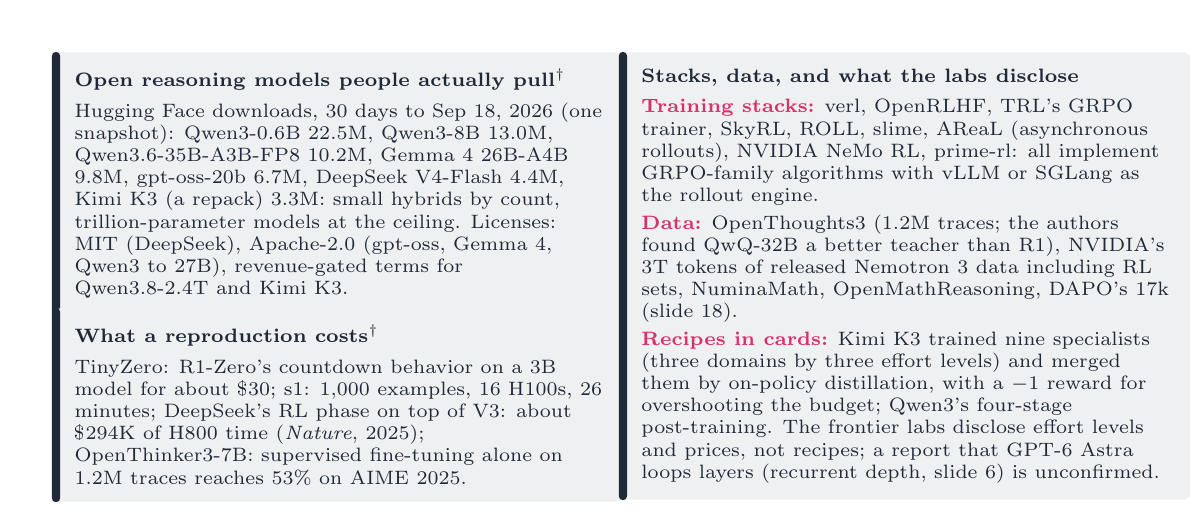
\begin{tikzpicture}
  \useasboundingbox (0,0) rectangle (14.4,5.9);
  \bgpanels{0.3}{5.6}{6.7cm}{Open reasoning models people actually pull$^\dagger$}{%
    Hugging Face downloads, 30 days to Sep 18, 2026 (one snapshot):
    Qwen3-0.6B 22.5M, Qwen3-8B 13.0M, Qwen3.6-35B-A3B-FP8 10.2M, Gemma 4
    26B-A4B 9.8M, gpt-oss-20b 6.7M, DeepSeek V4-Flash 4.4M, Kimi K3 (a
    repack) 3.3M: small hybrids by count, trillion-parameter models at
    the ceiling.
    Licenses: MIT (DeepSeek), Apache-2.0 (gpt-oss, Gemma 4, Qwen3 to
    27B), revenue-gated terms for Qwen3.8-2.4T and Kimi K3.}
  \bgpanels{0.3}{2.35}{6.7cm}{What a reproduction costs$^\dagger$}{%
    TinyZero: R1-Zero's countdown behavior on a 3B model for about
    \$30; s1: 1{,}000 examples, 16 H100s, 26 minutes; DeepSeek's RL
    phase on top of V3: about \$294K of H800 time (\emph{Nature},
    2025); OpenThinker3-7B: supervised fine-tuning alone on 1.2M traces
    reaches 53\% on AIME 2025.}
  \bgpanels{7.5}{5.6}{6.7cm}{Stacks, data, and what the labs disclose}{%
    \hl{outc}{Training stacks:} verl, OpenRLHF, TRL's GRPO trainer, SkyRL,
    ROLL, slime, AReaL (asynchronous rollouts), NVIDIA NeMo RL, prime-rl:
    all implement GRPO-family algorithms with vLLM or SGLang as the
    rollout engine.\\[2pt]
    \hl{outc}{Data:} OpenThoughts3 (1.2M traces; the authors found
    QwQ-32B a better teacher than R1), NVIDIA's 3T tokens of released
    Nemotron 3 data including RL sets, NuminaMath, OpenMathReasoning,
    DAPO's 17k (slide 18).\\[2pt]
    \hl{outc}{Recipes in cards:} Kimi K3 trained nine specialists (three
    domains by three effort levels) and merged them by on-policy
    distillation, with a $-1$ reward for overshooting the budget; Qwen3's
    four-stage post-training. The frontier labs disclose effort levels
    and prices, not recipes; a report that GPT-6 Astra loops layers
    (recurrent depth, slide 6) is unconfirmed.}
\end{tikzpicture}
\end{frame}

% ---------------------------------------------------------------- 25
\begin{frame}{Benchmarks and competitions: saturation, harness sensitivity}
\framesubtitle{The 2024 tests are solved; the field moved to agentic tasks, cost per task, and competitions graded by humans.}
\centering
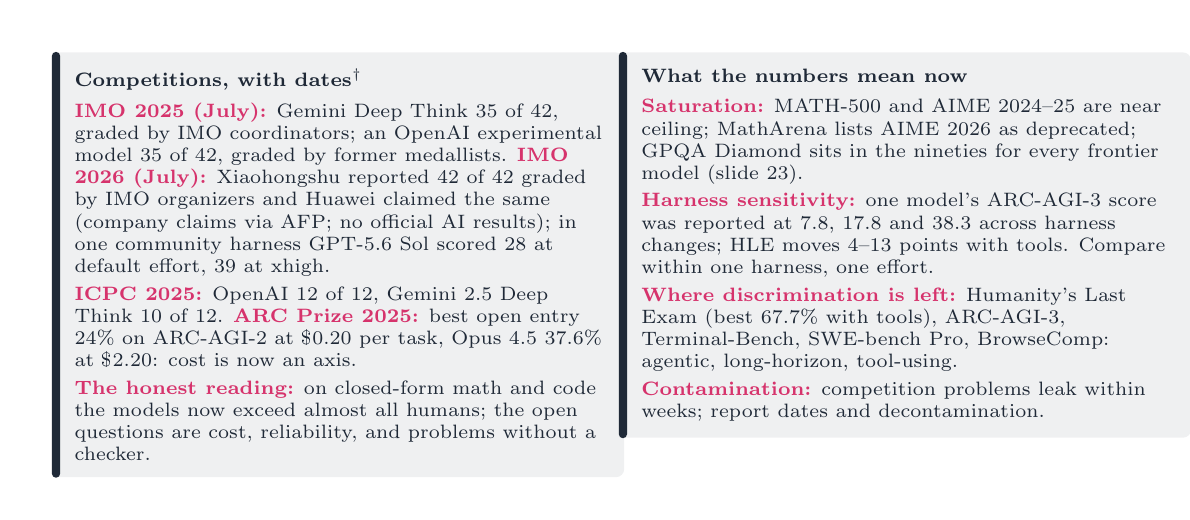
\begin{tikzpicture}
  \useasboundingbox (0,0) rectangle (14.4,5.9);
  \bgpanels{0.3}{5.6}{6.7cm}{Competitions, with dates$^\dagger$}{%
    \hl{outc}{IMO 2025 (July):} Gemini Deep Think 35 of 42, graded by
    IMO coordinators; an OpenAI experimental model 35 of 42, graded by
    former medallists. \hl{outc}{IMO 2026 (July):} Xiaohongshu reported
    42 of 42 graded by IMO organizers and Huawei claimed the same
    (company claims via AFP; no official AI results); in one community
    harness GPT-5.6 Sol scored 28 at default effort, 39 at xhigh.\\[2pt]
    \hl{outc}{ICPC 2025:} OpenAI 12 of 12, Gemini 2.5 Deep Think 10 of
    12. \hl{outc}{ARC Prize 2025:} best open entry 24\% on ARC-AGI-2 at
    \$0.20 per task, Opus 4.5 37.6\% at \$2.20: cost is now an axis.\\[2pt]
    \hl{outc}{The honest reading:} on closed-form math and code the
    models now exceed almost all humans; the open questions are cost,
    reliability, and problems without a checker.}
  \bgpanels{7.5}{5.6}{6.7cm}{What the numbers mean now}{%
    \hl{outc}{Saturation:} MATH-500 and AIME 2024--25 are near ceiling;
    MathArena lists AIME 2026 as deprecated; GPQA Diamond sits in the
    nineties for every frontier model (slide 23).\\[2pt]
    \hl{outc}{Harness sensitivity:} one model's ARC-AGI-3 score was
    reported at 7.8, 17.8 and 38.3 across harness changes; HLE moves
    4--13 points with tools. Compare within one harness, one effort.\\[2pt]
    \hl{outc}{Where discrimination is left:} Humanity's Last Exam (best
    67.7\% with tools), ARC-AGI-3, Terminal-Bench, SWE-bench Pro,
    BrowseComp: agentic, long-horizon, tool-using.\\[2pt]
    \hl{outc}{Contamination:} competition problems leak within weeks;
    report dates and decontamination.}
\end{tikzpicture}
\end{frame}

% ---------------------------------------------------------------- 26
\stage{9}
\begin{frame}{Where the chains break: brittle, jagged, confidently wrong}
\framesubtitle{The same problem in a different coat, a harness limit mistaken for a ceiling, and calibration that cuts both ways.}
\centering
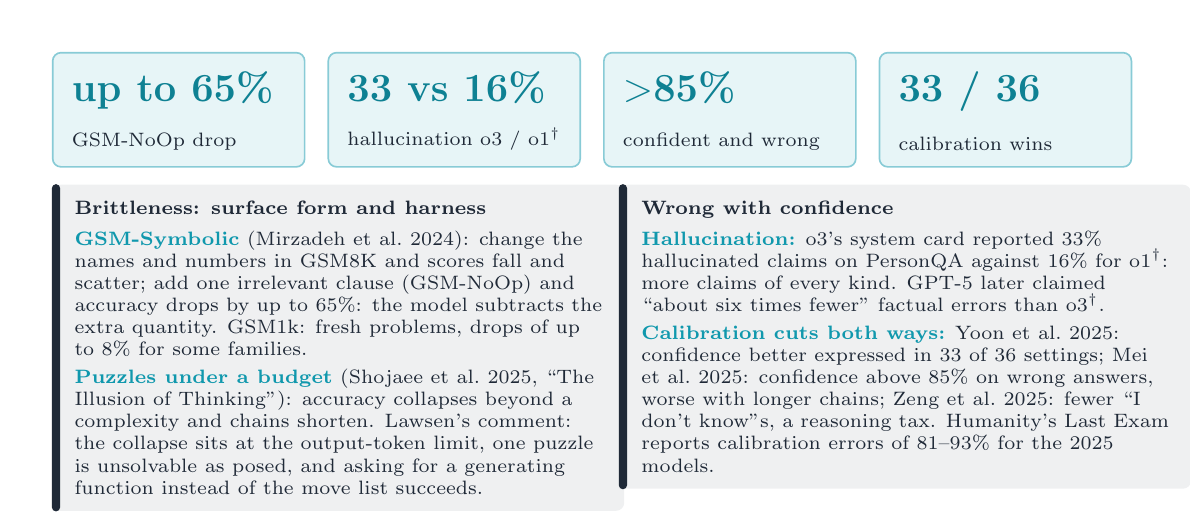
\begin{tikzpicture}
  \useasboundingbox (0,0) rectangle (14.4,5.9);
  \stat{0.3}{5.6}{up to 65\%}{GSM-NoOp drop}{vc}
  \stat{3.8}{5.6}{33 vs 16\%}{hallucination o3 / o1$^\dagger$}{vc}
  \stat{7.3}{5.6}{$>$85\%}{confident and wrong}{vc}
  \stat{10.8}{5.6}{33 / 36}{calibration wins}{vc}
  \bgpanels{0.3}{3.92}{6.7cm}{Brittleness: surface form and harness}{%
    \hl{vc}{GSM-Symbolic} (Mirzadeh et al.\ 2024): change the names and
    numbers in GSM8K and scores fall and scatter; add one irrelevant
    clause (GSM-NoOp) and accuracy drops by up to 65\%: the model
    subtracts the extra quantity. GSM1k: fresh problems, drops of up
    to 8\% for some families.\\[2pt]
    \hl{vc}{Puzzles under a budget} (Shojaee et al.\ 2025, ``The Illusion
    of Thinking''): accuracy collapses beyond a complexity and chains
    shorten. Lawsen's comment: the collapse sits at the output-token
    limit, one puzzle is unsolvable as posed, and asking for a generating
    function instead of the move list succeeds.}
  \bgpanels{7.5}{3.92}{6.7cm}{Wrong with confidence}{%
    \hl{vc}{Hallucination:} o3's system card reported 33\% hallucinated
    claims on PersonQA against 16\% for o1$^\dagger$: more claims of
    every kind. GPT-5 later claimed ``about six times fewer'' factual
    errors than o3$^\dagger$.\\[2pt]
    \hl{vc}{Calibration cuts both ways:} Yoon et al.\ 2025: confidence
    better expressed in 33 of 36 settings; Mei et al.\ 2025: confidence
    above 85\% on wrong answers, worse with longer chains; Zeng et al.\
    2025: fewer ``I don't know''s, a reasoning tax. Humanity's Last Exam
    reports calibration errors of 81--93\% for the 2025 models.}
\end{tikzpicture}
\end{frame}

% ---------------------------------------------------------------- 27
\begin{frame}{Safety: the chain as a window, and how it closes}
\framesubtitle{A legible chain lets a monitor catch misbehaviour; optimizing against the monitor, or against length, hides it again.}
\centering
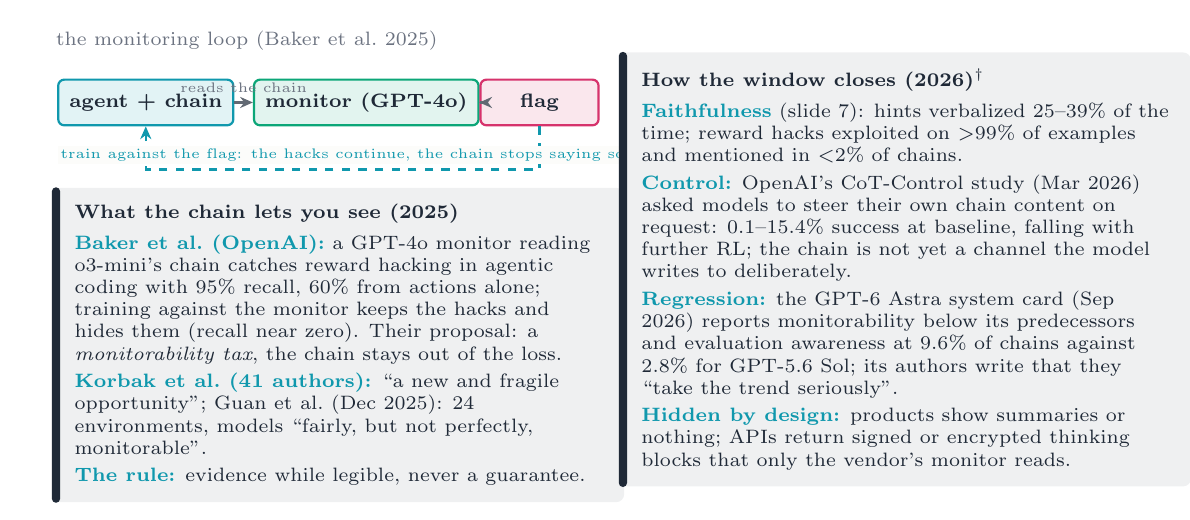
\begin{tikzpicture}
  \useasboundingbox (0,0) rectangle (14.4,5.9);
  % monitor loop diagram
  \node[lab,anchor=south west] at (0.3,5.55) {the monitoring loop (Baker et al.\ 2025)};
  \node[comp=vc,minimum width=2.2cm,minimum height=0.58cm,font=\scriptsize\bfseries,text=ink] (ag) at (1.5,4.95) {agent + chain};
  \node[comp=emb,minimum width=2.2cm,minimum height=0.58cm,font=\scriptsize\bfseries,text=ink] (mo) at (4.3,4.95) {monitor (GPT-4o)};
  \node[comp=outc,minimum width=1.5cm,minimum height=0.58cm,font=\scriptsize\bfseries,text=ink] (fl) at (6.5,4.95) {flag};
  \draw[flow] (ag) -- node[above,font=\tiny,text=muted] {reads the chain} (mo);
  \draw[flow] (mo) -- (fl);
  \draw[flow,draw=vc,dashed] (fl.south) |- (4.0,4.1) -| (ag.south);
  \node[font=\tiny,text=vc,anchor=south,fill=paper,inner sep=1pt] at (4.0,4.16) {train against the flag: the hacks continue, the chain stops saying so};
  \bgpanels{0.3}{3.88}{6.7cm}{What the chain lets you see (2025)}{%
    \hl{vc}{Baker et al.\ (OpenAI):} a GPT-4o monitor reading o3-mini's
    chain catches reward hacking in agentic coding with 95\% recall,
    60\% from actions alone; training against the monitor keeps the
    hacks and hides them (recall near zero). Their proposal: a
    \emph{monitorability tax}, the chain stays out of the loss.\\[2pt]
    \hl{vc}{Korbak et al.\ (41 authors):} ``a new and fragile
    opportunity''; Guan et al.\ (Dec 2025): 24 environments, models
    ``fairly, but not perfectly, monitorable''.\\[2pt]
    \hl{vc}{The rule:} evidence while legible, never a guarantee.}
  \bgpanels{7.5}{5.6}{6.7cm}{How the window closes (2026)$^\dagger$}{%
    \hl{vc}{Faithfulness} (slide 7): hints verbalized 25--39\% of the time;
    reward hacks exploited on $>$99\% of examples and mentioned in
    $<$2\% of chains.\\[2pt]
    \hl{vc}{Control:} OpenAI's CoT-Control study (Mar 2026) asked models to
    steer their own chain content on request: 0.1--15.4\% success at
    baseline, falling with further RL; the chain is not yet a channel the
    model writes to deliberately.\\[2pt]
    \hl{vc}{Regression:} the GPT-6 Astra system card (Sep 2026) reports
    monitorability below its predecessors and evaluation awareness at
    9.6\% of chains against 2.8\% for GPT-5.6 Sol; its authors write that
    they ``take the trend seriously''.\\[2pt]
    \hl{vc}{Hidden by design:} products show summaries or nothing; APIs
    return signed or encrypted thinking blocks that only the vendor's
    monitor reads.}
\end{tikzpicture}
\end{frame}

% ---------------------------------------------------------------- 28
\stage{10}
\begin{frame}{What is settled and what is contested, October 2026}
\framesubtitle{Two years of results sort into things every lab now relies on and questions the papers still argue about.}
\centering
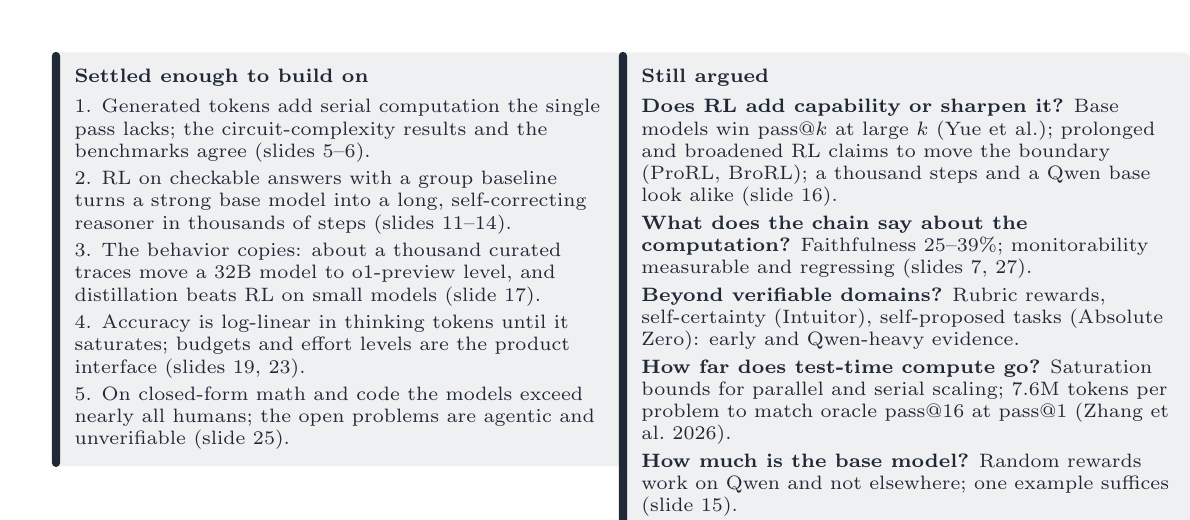
\begin{tikzpicture}
  \useasboundingbox (0,0) rectangle (14.4,5.9);
  \bgpanels{0.3}{5.6}{6.7cm}{Settled enough to build on}{%
    1. Generated tokens add serial computation the single pass lacks;
    the circuit-complexity results and the benchmarks agree (slides
    5--6).\\[2pt]
    2. RL on checkable answers with a group baseline turns a strong base
    model into a long, self-correcting reasoner in thousands of steps
    (slides 11--14).\\[2pt]
    3. The behavior copies: about a thousand curated traces move a 32B
    model to o1-preview level, and distillation beats RL on small models
    (slide 17).\\[2pt]
    4. Accuracy is log-linear in thinking tokens until it saturates;
    budgets and effort levels are the product interface (slides 19,
    23).\\[2pt]
    5. On closed-form math and code the models exceed nearly all
    humans; the open problems are agentic and unverifiable (slide 25).}
  \bgpanels{7.5}{5.6}{6.7cm}{Still argued}{%
    \hl{ink}{Does RL add capability or sharpen it?} Base models win
    pass@$k$ at large $k$ (Yue et al.); prolonged and broadened RL
    claims to move the boundary (ProRL, BroRL); a thousand steps and a
    Qwen base look alike (slide 16).\\[2pt]
    \hl{ink}{What does the chain say about the computation?}
    Faithfulness 25--39\%; monitorability measurable and regressing
    (slides 7, 27).\\[2pt]
    \hl{ink}{Beyond verifiable domains?} Rubric rewards, self-certainty
    (Intuitor), self-proposed tasks (Absolute Zero): early and
    Qwen-heavy evidence.\\[2pt]
    \hl{ink}{How far does test-time compute go?} Saturation bounds for
    parallel and serial scaling; 7.6M tokens per problem to match oracle
    pass@16 at pass@1 (Zhang et al.\ 2026).\\[2pt]
    \hl{ink}{How much is the base model?} Random rewards work on Qwen
    and not elsewhere; one example suffices (slide 15).}
\end{tikzpicture}
\end{frame}

% ---------------------------------------------------------------- 29
\begin{frame}{In practice: using one, training one, evaluating one}
\framesubtitle{Rules that follow from the lecture; the numbers are orders of magnitude, from the papers and cards cited.}
\centering
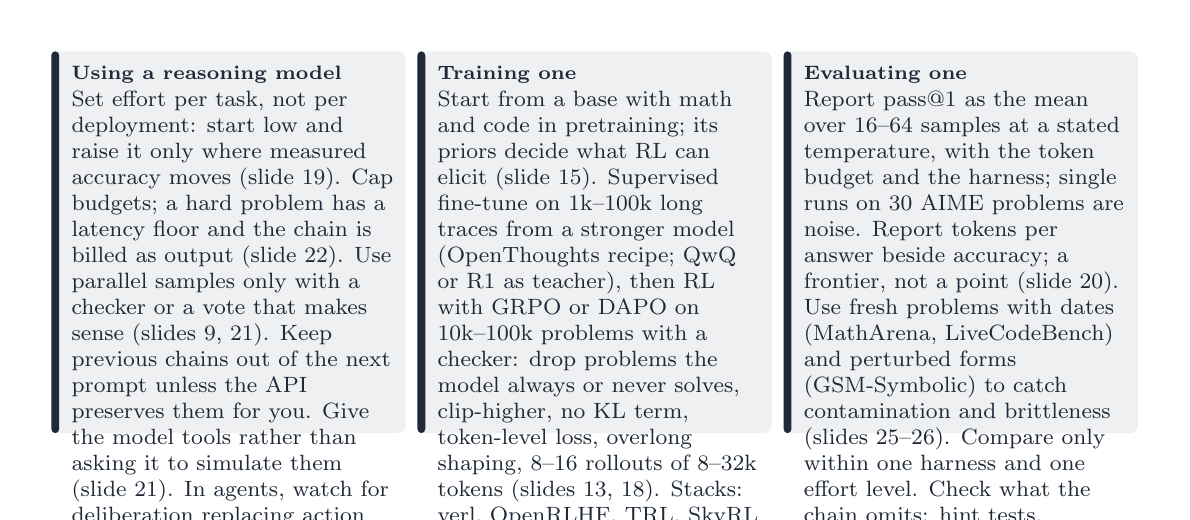
\begin{tikzpicture}
  \useasboundingbox (0,0) rectangle (14.4,5.9);
  \foreach \x/\c/\ttl/\body in {
      0.3/ink/{Using a reasoning model}/{Set effort per task, not per deployment: start low and raise it only where measured accuracy moves (slide 19). Cap budgets; a hard problem has a latency floor and the chain is billed as output (slide 22). Use parallel samples only with a checker or a vote that makes sense (slides 9, 21). Keep previous chains out of the next prompt unless the API preserves them for you. Give the model tools rather than asking it to simulate them (slide 21). In agents, watch for deliberation replacing action (slide 20). Treat the visible chain as a summary, not a log (slide 27).},
      4.95/ink/{Training one}/{Start from a base with math and code in pretraining; its priors decide what RL can elicit (slide 15). Supervised fine-tune on 1k--100k long traces from a stronger model (OpenThoughts recipe; QwQ or R1 as teacher), then RL with GRPO or DAPO on 10k--100k problems with a checker: drop problems the model always or never solves, clip-higher, no KL term, token-level loss, overlong shaping, 8--16 rollouts of 8--32k tokens (slides 13, 18). Stacks: verl, OpenRLHF, TRL, SkyRL (slide 24). Budgets: \$30 for a 3B toy, about \$1k for a 32B SFT run, \$300k for an R1-scale RL phase$^\dagger$.},
      9.6/ink/{Evaluating one}/{Report pass@1 as the mean over 16--64 samples at a stated temperature, with the token budget and the harness; single runs on 30 AIME problems are noise. Report tokens per answer beside accuracy; a frontier, not a point (slide 20). Use fresh problems with dates (MathArena, LiveCodeBench) and perturbed forms (GSM-Symbolic) to catch contamination and brittleness (slides 25--26). Compare only within one harness and one effort level. Check what the chain omits: hint tests, reward-hacking probes, calibration on wrong answers (slides 7, 26--27).}}{
    \fill[\c!7,rounded corners=3pt] (\x,0.75) rectangle (\x+4.5,5.6);
    \fill[\c,rounded corners=1.5pt] (\x,0.75) rectangle (\x+0.1,5.6);
    \node[anchor=north west,font=\scriptsize\bfseries,text=\c,inner sep=0,text width=4.1cm] at (\x+0.25,5.42) {\ttl};
    \node[anchor=north west,font=\fontsize{7.7}{9.4}\selectfont,text=ink,inner sep=0,text width=4.1cm,align=flush left] at (\x+0.25,5.1) {\body};}
\end{tikzpicture}
\end{frame}

% ---------------------------------------------------------------- 30
\begin{frame}{Summary: what to take from this lecture}
\framesubtitle{A reasoning model is a training recipe and an inference budget on the same transformer; both are now public.}
\centering
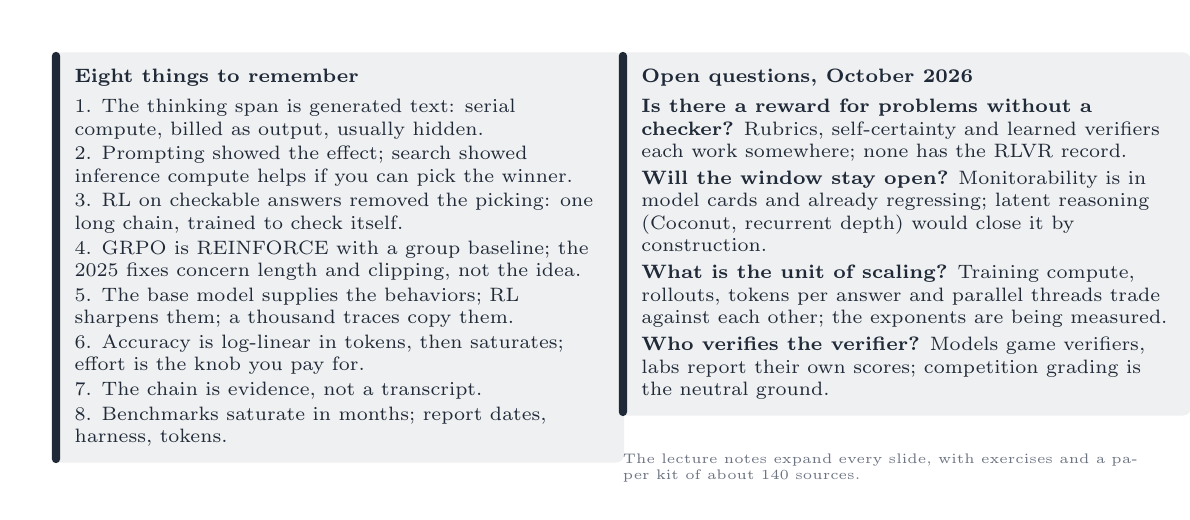
\begin{tikzpicture}
  \useasboundingbox (0,0) rectangle (14.4,5.9);
  \bgpanels{0.3}{5.6}{6.7cm}{Eight things to remember}{%
    1. The thinking span is generated text: serial compute, billed as
    output, usually hidden.\\[1pt]
    2. Prompting showed the effect; search showed inference compute
    helps if you can pick the winner.\\[1pt]
    3. RL on checkable answers removed the picking: one long chain,
    trained to check itself.\\[1pt]
    4. GRPO is REINFORCE with a group baseline; the 2025 fixes concern
    length and clipping, not the idea.\\[1pt]
    5. The base model supplies the behaviors; RL sharpens them; a
    thousand traces copy them.\\[1pt]
    6. Accuracy is log-linear in tokens, then saturates; effort is the
    knob you pay for.\\[1pt]
    7. The chain is evidence, not a transcript.\\[1pt]
    8. Benchmarks saturate in months; report dates, harness, tokens.}
  \bgpanels{7.5}{5.6}{6.7cm}{Open questions, October 2026}{%
    \hl{ink}{Is there a reward for problems without a checker?} Rubrics,
    self-certainty and learned verifiers each work somewhere; none has
    the RLVR record.\\[2pt]
    \hl{ink}{Will the window stay open?} Monitorability is in model cards
    and already regressing; latent reasoning (Coconut, recurrent depth)
    would close it by construction.\\[2pt]
    \hl{ink}{What is the unit of scaling?} Training compute, rollouts,
    tokens per answer and parallel threads trade against each other;
    the exponents are being measured.\\[2pt]
    \hl{ink}{Who verifies the verifier?} Models game verifiers, labs
    report their own scores; competition grading is the neutral ground.}
  \node[lab,anchor=north west,text width=6.7cm,font=\tiny] at (7.5,0.55) {The lecture notes expand every slide, with exercises and a paper kit of about 140 sources.};
\end{tikzpicture}
\end{frame}

% ---------------------------------------------------------------- 31
\begin{frame}{Sources}
\framesubtitle{Papers by thread, then vendor material and community posts; $^\dagger$ marks vendor, press and community sources.}
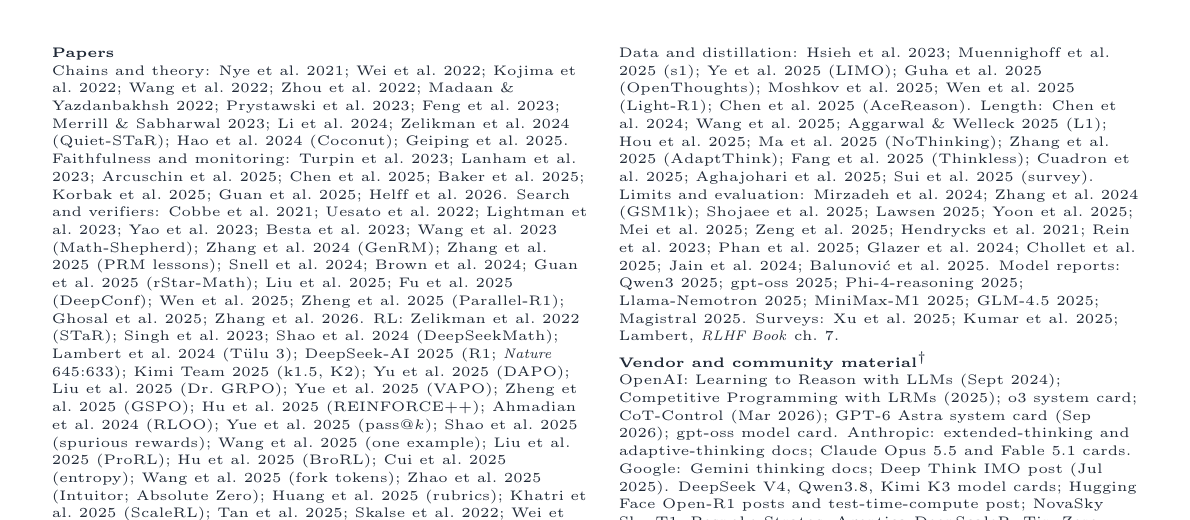
\begin{tikzpicture}
  \useasboundingbox (0,0) rectangle (14.4,5.9);
  \node[anchor=north west,inner sep=0,text width=6.8cm,font=\fontsize{5.4}{6.4}\selectfont,text=ink,align=flush left] at (0.3,5.65) {%
    \textbf{Papers}\\
    Chains and theory: Nye et al.\ 2021; Wei et al.\ 2022; Kojima et al.\ 2022; Wang et al.\ 2022; Zhou et al.\ 2022; Madaan \& Yazdanbakhsh 2022; Prystawski et al.\ 2023; Feng et al.\ 2023; Merrill \& Sabharwal 2023; Li et al.\ 2024; Zelikman et al.\ 2024 (Quiet-STaR); Hao et al.\ 2024 (Coconut); Geiping et al.\ 2025. Faithfulness and monitoring: Turpin et al.\ 2023; Lanham et al.\ 2023; Arcuschin et al.\ 2025; Chen et al.\ 2025; Baker et al.\ 2025; Korbak et al.\ 2025; Guan et al.\ 2025; Helff et al.\ 2026. Search and verifiers: Cobbe et al.\ 2021; Uesato et al.\ 2022; Lightman et al.\ 2023; Yao et al.\ 2023; Besta et al.\ 2023; Wang et al.\ 2023 (Math-Shepherd); Zhang et al.\ 2024 (GenRM); Zhang et al.\ 2025 (PRM lessons); Snell et al.\ 2024; Brown et al.\ 2024; Guan et al.\ 2025 (rStar-Math); Liu et al.\ 2025; Fu et al.\ 2025 (DeepConf); Wen et al.\ 2025; Zheng et al.\ 2025 (Parallel-R1); Ghosal et al.\ 2025; Zhang et al.\ 2026. RL: Zelikman et al.\ 2022 (STaR); Singh et al.\ 2023; Shao et al.\ 2024 (DeepSeekMath); Lambert et al.\ 2024 (T\"ulu 3); DeepSeek-AI 2025 (R1; \emph{Nature} 645:633); Kimi Team 2025 (k1.5, K2); Yu et al.\ 2025 (DAPO); Liu et al.\ 2025 (Dr.\ GRPO); Yue et al.\ 2025 (VAPO); Zheng et al.\ 2025 (GSPO); Hu et al.\ 2025 (REINFORCE++); Ahmadian et al.\ 2024 (RLOO); Yue et al.\ 2025 (pass@$k$); Shao et al.\ 2025 (spurious rewards); Wang et al.\ 2025 (one example); Liu et al.\ 2025 (ProRL); Hu et al.\ 2025 (BroRL); Cui et al.\ 2025 (entropy); Wang et al.\ 2025 (fork tokens); Zhao et al.\ 2025 (Intuitor; Absolute Zero); Huang et al.\ 2025 (rubrics); Khatri et al.\ 2025 (ScaleRL); Tan et al.\ 2025; Skalse et al.\ 2022; Wei et al.\ 2025 (SWE-RL); Feng et al.\ 2025 (ReTool); Gou et al.\ 2023 (ToRA); Chen et al.\ 2025 (pass@$k$ training); Zhai et al.\ 2026; Cheng et al.\ 2026.};
  \node[anchor=north west,inner sep=0,text width=6.6cm,font=\fontsize{5.4}{6.4}\selectfont,text=ink,align=flush left] at (7.5,5.65) {%
    Data and distillation: Hsieh et al.\ 2023; Muennighoff et al.\ 2025 (s1); Ye et al.\ 2025 (LIMO); Guha et al.\ 2025 (OpenThoughts); Moshkov et al.\ 2025; Wen et al.\ 2025 (Light-R1); Chen et al.\ 2025 (AceReason). Length: Chen et al.\ 2024; Wang et al.\ 2025; Aggarwal \& Welleck 2025 (L1); Hou et al.\ 2025; Ma et al.\ 2025 (NoThinking); Zhang et al.\ 2025 (AdaptThink); Fang et al.\ 2025 (Thinkless); Cuadron et al.\ 2025; Aghajohari et al.\ 2025; Sui et al.\ 2025 (survey). Limits and evaluation: Mirzadeh et al.\ 2024; Zhang et al.\ 2024 (GSM1k); Shojaee et al.\ 2025; Lawsen 2025; Yoon et al.\ 2025; Mei et al.\ 2025; Zeng et al.\ 2025; Hendrycks et al.\ 2021; Rein et al.\ 2023; Phan et al.\ 2025; Glazer et al.\ 2024; Chollet et al.\ 2025; Jain et al.\ 2024; Balunovi\'c et al.\ 2025. Model reports: Qwen3 2025; gpt-oss 2025; Phi-4-reasoning 2025; Llama-Nemotron 2025; MiniMax-M1 2025; GLM-4.5 2025; Magistral 2025. Surveys: Xu et al.\ 2025; Kumar et al.\ 2025; Lambert, \emph{RLHF Book} ch.\ 7.\\[2pt]
    \textbf{Vendor and community material$^\dagger$}\\
    OpenAI: Learning to Reason with LLMs (Sept 2024); Competitive Programming with LRMs (2025); o3 system card; CoT-Control (Mar 2026); GPT-6 Astra system card (Sep 2026); gpt-oss model card. Anthropic: extended-thinking and adaptive-thinking docs; Claude Opus 5.5 and Fable 5.1 cards. Google: Gemini thinking docs; Deep Think IMO post (Jul 2025). DeepSeek V4, Qwen3.8, Kimi K3 model cards; Hugging Face Open-R1 posts and test-time-compute post; NovaSky Sky-T1; Bespoke-Stratos; Agentica DeepScaleR; TinyZero; MathArena; ARC Prize 2025 report; \emph{Scientific American} on R1's cost; AFP on IMO 2026; vendor pricing pages, all read Oct 21--22, 2026. Full list with arXiv identifiers in the paper kit.};
\end{tikzpicture}
\end{frame}
\end{document}
